\documentclass[a4paper,USenglish]{tex/lipics-v2016}

\usepackage{xspace,listings,url,framed,amssymb,
            amsmath,tex/mathpartir,hyperref,
            stmaryrd, graphicx % double brackets llbracket
}


%% Formatting
\newcommand{\EM}[1]{\ensuremath{#1}\xspace}
\newcommand{\xt}[1]{{\sf{#1}}}
\newcommand{\bt}[1]{\xt{\bf #1}}
\renewcommand{\b}[1]{\EM{\overline{#1}}}
\newcommand{\EMxt}[1]{\EM{\xt{#1}}}
\newcommand{\EMbt}[1]{\EM{\bt{#1}}}

%% Variables
\newcommand{\x}   {\EMxt x}
\newcommand{\n}   {\EMxt n}
\newcommand{\e}   {\EMxt e}
\newcommand{\m}   {\EMxt m}
\newcommand{\s}   {\EM{\sigma}}
\renewcommand{\t} {\EMxt t}
\newcommand{\ta}  {\EM{\tau}}
\renewcommand{\a} {\EMxt a}
\newcommand{\K}   {\EMxt K}
\renewcommand{\k} {\EMxt k}
\newcommand{\Kp}  {{\EMxt{K'}}}
\newcommand{\Kpp}  {{\EMxt{K''}}}
\newcommand{\Kppp}  {{\EMxt{K'''}}}
\newcommand{\ep}  {{{\EMxt{e'}}}}
\newcommand{\epp}  {{{\EMxt{e''}}}}
\renewcommand{\sp}{{{\EM{\s'}}}}
\newcommand{\spp}{{{\EM{\s''}}}}
\newcommand{\ap}  {\EM{\a'}}
\newcommand{\aE}[1]  {\EM{\a_{#1}}}
\newcommand{\app}  {\EM{\a''}}
\newcommand{\tp}  {\EM{ \t'}}
\newcommand{\tpp}  {\EM{ \t''}}
\newcommand{\C}   {\EMxt C}
\newcommand{\Cp}  {\EMxt{C'}}
\newcommand{\EC}   {\EMxt E}
\newcommand{\fd}  {\EMxt{fd}}
\newcommand{\md}  {\EMxt{md}}
\newcommand{\mdpp}  {\EM{\md'}}
\newcommand{\mt}  {\EMxt{mt}}
\newcommand{\mtp}  {\EMxt{mt'}}
\newcommand{\mtpp}  {\EMxt{mt''}}
\newcommand{\M}{\EMxt M}
\newcommand{\MN}  {\EMxt{M\,K}}
\newcommand{\MNargs}[1]  {\EMxt {M #1~K}}
\newcommand{\f}   {\EMxt f}
\newcommand{\fp}   {\EMxt{ f'}}
\newcommand{\E}   {\EM{\Gamma}}
\newcommand{\EE}   {\EM{\mathcal{E}}}
\newcommand{\any} {\EM{\star}}
\newcommand{\this}{\EMxt{this}}
\newcommand{\that}{\EMxt{that}}
\newcommand{\none}{\EM{\cdot}}
\newcommand{\D}   {\EMxt D}
\newcommand{\Dp}   {\EMxt{D'}}
\newcommand{\p}   {\EMxt p}
\newcommand{\np}{\n'}

\newcommand{\Get}[2]   {\EM{#1.#2()}}
\newcommand{\Set}[3]   {\EM{#1.#2(#3)}}
\newcommand{\Call}[3]  {\EM{#1.#2(#3)}}
\newcommand{\DynCall}[3]  {\EM{#1@#2(#3)}}

\newcommand{\New}[2]   {\EM{\new\;#1(#2)}}
\newcommand{\SubCast}[2]{\EM{<\hspace{-.6mm}{#1}\hspace{-.6mm}>\hspace{-1mm}\;{#2}}}
\newcommand{\ShaCast}[2]{\EM{\prec #1 \succ #2}}
\newcommand{\MonCast}[2]{\EM{\triangleleft\; #1 \triangleright #2}}
\newcommand{\BehCast}[2]{\EM{\blacktriangleleft #1 \blacktriangleright #2}}
\newcommand{\new}      {\EM{\bt{new}}}
\newcommand{\HT}[2]    {\EM{{#1}\!:{#2}}}
\newcommand{\Mdef}[5]  {\EM{ \HT{ #1( \HT{#2}{#3})}{#4}\;\{{#5}\}}}
\newcommand{\Mdefz}[3] {\EM{ \HT{ #1()}{#2}\;\{{#3}\}}}
\newcommand{\Mdefa}[4]  {\EM{ \HT{ #1( #2 )}{#3}~\{{#4}\}}}
\newcommand{\obj}[2]   { \EM{ #1\{#2\}}}
\newcommand{\alloc}[4] {\EM{#1\;#2  = \xt{alloc}(#3, #4)}}
\newcommand{\cast}[8]  {\EM{#6\;#7\;#8=\xt{#5 cast}(#1, #2, #3, #4)}}
\newcommand{\behcast}[7]  {\EM{\xt{behcast}(#1, #2, #3, #4)=#5\,#6\,#7}}
\newcommand{\moncast}[6]  {\EM{\xt{moncast}(#1, #2, #3, #4)=#5\,#6}}

\newcommand{\Alt}[1]   { &\B #1 \\}
\newcommand{\B}        {\EM{~|~}}
\newcommand{\bang}     {\EM{\xt{!}}}

\newcommand{\dispatch}[5] {\EM{#1\;#2 = \xt{disp}(#3,#4,#5)}}
\newcommand{\readf}[4]{\EM{\xt{read}(#1,#2,#3,#4)}}
\newcommand{\convert}[1]{\EM{\xt{cnvtMD}(#1)}}
\newcommand{\convertFD}[1]{\EM{\xt{cnvtFD}(#1)}}
\newcommand{\readfield}[4]{\EM{#1 = \xt{read}(#2,#3,#4)}}
\newcommand{\setf}[5] {\EM{\xt{write}(#1,#2,#3,#4,#5)}}
\newcommand{\Reduce}[6]   {\EM{{#1}~{#2}~{#3} \rightarrow {#4}~{#5}~{#6}}}
\newcommand{\ReduceA}[6]  {\EM{#1~#2~#3 } & \EM{\rightarrow #4~#5~#6}}
\newcommand{\Class}[3]    {\EM{\bt{class}\;#1\,\{\,#2~#3\,\}}}
\newcommand{\Ftype}[2]    {\EM{ \HT{#1}{#2} }}
\newcommand{\Fdef}[2]    {\EM{ \HT{#1}{#2} }}
\newcommand{\Mtype}[3]    {\EM{ \HT{#1(#2)}{#3}}}
\newcommand{\Type}[1]     {\EM{\{#1\}}}

\newcommand{\opdef}[2]    {\framebox[1.1\width]{#1} ~ #2\\}
\newcommand{\Map}[2]     {\EM{ #1[#2] }}
\newcommand{\Bind}[2]     {\EM{#1 \mapsto #2}}

\newcommand{\Sub}{\EM{<:}}
\newcommand{\OK}{\EM{~\checkmark}}
\newcommand{\SubE}[1]{\EM{<:_{#1}}}
\newcommand{\names}[1]{\EM{\xt{names}(#1)}}
\newcommand{\untyped}[1]{\EM{\xt{untyped}(#1)}}

\newcommand{\mnames}[1]{\EM{\xt{methName}(#1)}}
\newcommand{\fnames}[1]{\EM{\xt{fieldName}(#1)}}


\newcommand{\ConsSub}{\EM{\lesssim}}

\newcommand{\CondRule}[3]{ #3 &~ #2 \\}
\newcommand{\SuchRule}[3]{ #3 &~{\emph{s.t.}} #2 \\}
\newcommand{\EnvType}[5]{ \EM{#1\,#2\,#3\vdash #4 : #5}}

\newcommand{\IRule}[4][]{\inferrule*[lab={\tiny #2},#1]{#3}{#4}}
\newcommand{\HasType}[3]{ \EM{#1 (#2) = #3}}
\newcommand{\wrapper}[1]{\EM{\xt{wrap}(#1)}}
\newcommand{\spec}[4]{\EM{\xt{spec}(#1,#2,#3,#4)}}

\newcommand{\castfn}[4]{\text{cast}(#1,#2,#3,#4)}
\newcommand{\GenCast}[5]{#1~#2 \vdash #3 \hookrightarrow #4 \Uparrow #5 }
\newcommand{\AnaCast}[5]{#1~#2 \vdash #3 \Downarrow #5 \hookrightarrow #4}
\newcommand{\TransClass}[2]{\EM{ #1 \rightharpoonup #2 }}
\newcommand{\inv}[2]{\xt{invoke}(#1, #2)}
\newcommand{\classoff}[2]{\EM{\xt{mtypes}(#1,#2)}}
\newcommand{\classoffs}[3]{\EM{\xt{mtypes}(#1,#2,#3)}}
\newcommand{\mtype}[3]{\EM{\xt{mtype}(#1,#2,#3)}}
\newcommand{\wftype}[3]{\EM{\xt{wftype}(#1,#2,#3)}}

\newcommand{\field}[2]{\EM{\xt{field}(#1,#2)}}
\newcommand{\In}{\EM{\in}}

\newcommand{\T}{\EM{\xt T}}
\newcommand{\Cast}{Cast }
\newcommand{\fb}{\EM{\xt{f!}}}

\newcommand{\AND}{\EM{\wedge}}
\newcommand{\App}[2]{\EM{#1(#2)}}

\newcommand{\StrSub}[4]{\EM{#1~#2\vdash #3\Sub #4}}
\newcommand{\tmeet}[4]{\xt{tmeet}(#1,#2,#3,#4)}
\newcommand{\mmeet}[4]{\xt{mmeet}(#1,#2,#3,#4)}
\newcommand{\mtypes}[2]{\xt{mtypes}(#1,#2)}


\newcommand{\WFtype}[2]{\EM{#1\vdash#2 \OK}}
\newcommand{\WF}[4]{\EM{#1\,#2\,#3\vdash#4 \OK}}
\newcommand{\WFp}[3]{#1~#2~#3\OK}

\renewcommand{\P}{\EMxt P}
\newcommand{\Pp}{\EMxt{P'}}


\newcommand{\retype}[5]{\xt{retype}(#1,#2,#3,#4,#5)}
\newcommand{\htype}[3]{\EM{\xt{htype}(#1,#2,#3)}}
\newcommand{\ftypes}[4]{\xt{ftypes}(#1,#2,#3,#4)}
\newcommand{\typeof}[1]{\xt{typeOf}(#1)}
\newcommand{\classgen}[1]{\xt{classgen}(#1)}
\renewcommand{\S}{\EM{\tau}}
\newcommand{\Sp}{\EM{\tau'}}
\newcommand{\Spp}{\EM{\tau''}}
\newcommand{\EQ}{\EM{\equiv}}

\newcommand{\Dom}[1]{\EM{\xt{dom}(#1)}}
\newcommand{\fresh}[1]{\EM{#1~\xt{fresh}}}

\newcommand{\progtrans}[2]{#1 ~\hookrightarrow_p~ #2}
\newcommand{\classtrans}[3]{#1 \vdash #2 ~\hookrightarrow_c~ #3}
\newcommand{\methtrans}[4]{#1~#2 \vdash #3 ~\hookrightarrow_m~ #4}
\newcommand{\statictype}[2]{\xt{static}(#1,#2)}


\usepackage[textsize=tiny]{todonotes}
% Author macros::begin %%%%%%%%%%%%%%%%%%%%%%%%%%%%%%%%%%%%%%%%%%%%%%%%
\title{On Gradual Type Systems for Objects}
\titlerunning{Gradual Typing for Objects, Redux}
%% provide for each author the \author and \affil macro, even if same
\author[1]{Anonymous}
\affil[1]{}
\authorrunning{Anon} %mandatory. First: Use abbreviated first/middle names. Second (only in severe cases): Use first author plus 'et. al.'
\Copyright{Anon}%mandatory, please use full first names. LIPIcs license is "CC-BY";  http://creativecommons.org/licenses/by/3.0/
%\subjclass{Dummy classification -- please refer to \url{http://www.acm.org/about/class/ccs98-html}}% mandatory: Please choose ACM 1998 classifications from http://www.acm.org/about/class/ccs98-html . E.g., cite as "F.1.1 Models of Computation". 
%\keywords{Dummy keyword -- please provide 1--5 keywords}% mandatory: Please provide 1-5 keywords
% Author macros::end %%%%%%%%%%%%%%%%%%%%%%%%%%%%%%%%%%%%%%%%%%%%%%%%%

%Editor-only macros:: begin (do not touch as author)%%%%%%%%
\EventEditors{Anon}
\EventNoEds{2}
\EventLongTitle{}
\EventShortTitle{ECOOP 2017}
\EventAcronym{ECOOP}
\EventYear{2017}
\EventDate{}
\EventLocation{}
\EventLogo{}
\SeriesVolume{42}
\ArticleNo{23}
% Editor-only macros::end %%%%%%%%%%%%%%%%%%%%%%%%%%%%%%%%%%%%%%%%%%%%%%%


\begin{document}

%%%%%%%%%%%%%%%%%%%%%%%%%%%%%%%%%%%%%%%%%%%%%%%%%%%%%%%%%%%%%%%%%%%%%%%%%%%

\maketitle

%\begin{abstract}
%The popularity of dynamically typed languages has given rise to a cottage
%industry of type systems that provide various degrees of assurance
%while allowing some code to remain free of type annotations. 
%The motivation underlying these new type systems is that they give
%programmers a way to incrementally migrate a code base from untyped
%to typed.  It is becoming increasingly clear that the design of these
%type systems must carefully consider issues such expressiveness of the 
%annotation language, granularity of type regions, and performance overheads
%of any associated run-time checks.  This paper focuses on gradual types for 
%object-oriented languages and attempts to explain some of the key design 
%dimensions and trade-offs of three implemented gradual types systems.
%This is achieved by embedding the different design into a core calculus
%that is broadly representative of dynamic languages such as Python, JavaScript
%and Ruby.
%\end{abstract} 

\section{Introduction}
Well-typed programs go wrong every day. Short of programming with a proof
assistant, our programs will remain replete with errors that lead to
undesirable outcomes.  The question that face language designers is what
classes of errors are frequent enough that it makes sense to try to catch in
the programming language itself, and how much linguistic machinery to expose
to end-users for that purpose.  At one end of the spectrum, some of the most
popular languages of the day rely solely on dynamic checks to catch errors
as the program runs. Towards the other end, statically typed languages
expose a set of type annotations that programmers have to use in their code
and, in return, these languages ensure that many errors are ruled out entirely.

Gradual typing attempts to merge both of these world-views by allowing
developers to add annotations in an incremental manner, with the promise of
rewards in error prevention commensurate to the effort invested in selecting
where to put annotations. Types have other benefits, by making programmer
intent explicit, they play the role of simple machine-checked documentation,
and they also have the potential of providing useful information for
the compiler to generate efficient code.

This paper explores the design space of gradual type systems for
object-oriented languages. We aim to expose the main forces influencing the
design of practical systems, and to provide advice for the next generation
of gradually typed languages. To this end, we have designed a minimialistic
object-based language that supports statically and dynamically typed code
fragments. On top of this common core, we then build models of several
practical gradual type systems and illustrate their differences in terms of
catching errors. While our work has a formal flavor, we are careful to
discuss the practical implications of different choices in the light of
our experience with the implementation of several gradually typed systems.

The fundamental property that a type system object-based language should
guarantee is that an expression of the form 
\vspace{-1mm}\[ \xt{x.m(y)} \]

\vspace{-1mm}\noindent does not result in, to borrow Smalltalk terminology,
a \emph{message not understood} error.  That is to say, method \xt{m} exists
in the object bound to variable \x. Many static type systems only
provide a partial guarantee as they make an exception for \xt{null} or
\xt{undefined} references; the call may fail as the test whether \x is
bound to an object is deferred to execution.

At the heart of the design of a gradual type system lies the choice of
definition of \emph{soundness} and the static and dynamic mechanisms
employed to enforce it. The literature is ripe with proposals with subtly
different properties and mechanisms.  One key distinction is what it means
for a variable \x to be of type \T. In a traditional statically typed
language, \x will refer to either an instance of the class denoted by \T or
one of its sub-classes; we say that \T is a \emph{concrete type}. In some
proposals, a variable \x of type \T can refer to an instance of any class,
in this case we say that \T is \emph{unconstrained type}. Lastly, in some
systems \x is allowed to refer to any value but the language implementation
will ensure that the value behaves as if it was of type \T, we call this a
\emph{promised type}.

While statically typed languages such as Scala only offer concrete types and
dynamically typed languages like Python have a single, implicit,
unconstrained type, gradually typed language have experimented with various
combinations.  C\# has concrete typed but also support a single
unconstrained type \xt{dyn}~\cite{Bierman10}. Thorn~\cite{popl10} and
StrongScript~\cite{ecoop15} both support concrete types as well as
unconstrained types. Languages such as Facebook's Hack and
TypeScript~\cite{typescript13} support only unconstrained types.  Finally
Reticulated Python~\cite{siek14} and Typed Racket~\cite{tf-dls06} support
promised types.


\section{Inside the Cottages}
%explanation..

In this paper, we will look at gradual type systems that present each of the
above interpretations of gradual typing, some of which allow several at the 
same time. We begin with a discussion of Strongscript, a extension of Typescript
that provides \emph{concrete types} as well as \emph{unconstrained types}, then
examine Typed Racket, providing \emph{promised types}, and finish with a
discussion of two type systems avaliable for Reticulated Python, both offering
a different perspective on \emph{promised types}. 

\subsection{Strongscript}

Strongscript is an evolution of Typescript, an industrial unsound optional
typing approach for Javascript. Both Strongscript and Typescript aim to
offer a method for Javascript programmers to migrate their dynamic code
to typed code, but to discuss Strongscript, we first need to explain its 
basis in Typescript.

\begin{figure}[h]
\begin{verbatim}
class A { a() : number { return 0; } }
class B { b() : string { return "b"; } }

function test(x: A) {
  return x.a();
}
test(new B())
\end{verbatim}
\caption{Typescript Example 1: Static type error}
\label{fig:tsex1}
\end{figure}

Figure~\ref{fig:tsex1} presents a simple typed program that is statically 
rejected by Typescript, where we try to call a non-existent method on an object,
an issue which Typescript notices and rejects statically. Typescript did this
by noticing that the type A is not compatible with the type B.

However, consider figure~\ref{fig:tsex2}, where we place the instance of B
into an any-typed variable, then call test with that variable. Since the
semantics of this program are identical to the previous example, one could
expect that Typescript would notice the issue and report a static type
error. When we run the Typescript compiler, the program is accepted by the
compiler, and execution produces a ``message not understood'' error at the
invocation site on line 5, inside the function where we expected to see no
errors.

\begin{figure}[h]
\begin{verbatim}
class A { a() : number { return 0; } }
class B { b() : string { return "b"; } }

function test(x:A) {
	return x.a();
}
var evil:any = new B()
test(evil)
\end{verbatim}
\caption{Typescript Example 2: Dynamic type error}
\label{fig:tsex2}
\end{figure}

This issue goes undetected because Typescript \emph{only} checks the static
compatibility of types. It was able to tell that an A is not a B, but cannot
determine that the real value of \xt{evil} is incompatible with A. As a result,
Typescript provides no guarantee that a value inhabiting a type is actually of
that type, and therefore is unsound. The designers of Typescript made this choice
for two major reasons:

\begin{itemize}
\item Incorrect types do not create errors. Even if the program is
  ill-typed, yet ran before types were added, it will still run in typed
  configuration, albeit while breaking the programmer's type-based
  intuition. This allows programs to be typed more easily.
\item Not checking types at runtime incurs no runtime overhead. As discussed
  later, ensuring the type correctness of a program at runtime incurs a
  substantial performance penalty. By not having any runtime component,
  Typescript has the same performance as Javascript does.
\end{itemize}

Simply adding soundness to all types would run straight into both of these
issues, as it would cause running programs to stop working and would 
also incur runtime overhead. Strongscript sets out to add soundness to
Typescript, so it has to deal with these problems and coexist with this
\emph{unconstrained} ecosystem, while simultaneously preventing the issue
identified in figure~\ref{fig:tsex2}.

To provide soundness while still avoiding compatibility problems with 
Typescript, Strongscript provides programmers with a choice of type
safety guarantee - a programmer can choose to write \emph{unconstrained}
types (denoted $\t$, for compatibility with Typescript) or \emph{concrete}
types (denoted $\t\xt{!}$), sidestepping both problems with a fully sound
gradual typing system and devolving responsibility for the choice onto
the programmer.

\begin{figure}[h]
\begin{verbatim}
class A { a() : number { return 0; } }
class B { b() : string { return "b"; } }

function test(x : A!) {
  return x.a();
}
var evil:any = new B()
test(evil)
\end{verbatim}
\caption{Strongscript: Dynamic type error}
\label{fig:ssex}
\end{figure}

In figure~\ref{fig:ssex}, we have the same program that caused Typescript to
have a runtime type error, but with one key change: now, instead of taking
type $\xt{A}$, the function test takes type $\xt{A!}$, and therefore has a
soundness requirement. Like Typescript, Strongscript cannot reason about the
real value of evil statically - all it sees is that evil is of type $\any$,
and something of type $\any$ \emph{could} work with something expecting type
$\xt{A}$. As a result, this program is still allowed statically by
Strongscript.

To solve this problem and preserve type safety, Strongscript dynamically
checks that the argument is type correct. While we do not get a static type
error, when we try to run the program, we get a dynamic type error at line
8, where we try to pass a B where an A is expected.

In this manner, a programmer can use the Strongscript types to control
enforcement and the resulting restrictions on code in a gradually typed
program. However, Strongscript provides another interesting property that
relates the \emph{unconstrained} and the \emph{concrete} types, illustrated
in figure~\ref{fig:ssex}.

\begin{figure}[h]
\begin{verbatim}
class A { a() : number { return 0; } }
class B { b() : string { return "b"; } }

function test(x : A) {
  return x.a();
}
var nice:A = new A()
test(nice)
\end{verbatim}
\caption{Strongscript: Correct, unconstrained typed program}
\label{fig:ssex2}
\end{figure}

Here, in figure~\ref{fig:ssex2}, we have modified the previous examples to execute correctly and typecheck
successfully with only \emph{unconstrained} types. As a result, we can simply 
transform it into the program seen in figure~\ref{fig:ssex3} and no errors, runtime
or compile time, are produced.

\begin{figure}[h]
\begin{verbatim}
class A { a() : number { return 0; } }
class B { b() : string { return "b"; } }

function test(x : A) {
  return x.a();
}
var nice:A = new A()
test(nice)
\end{verbatim}
\caption{Strongscript: Correct, concretely typed program}
\label{fig:ssex3}
\end{figure}

The last property we will discuss about Strongscript is its use of 
\emph{concrete} types. Concrete gradual typing is based on \emph{type identity},
rather than \emph{type compatibility}, a topic we will discuss in the context of
Reticulated Python. To illustrate this, consider figure~\ref{fig:ssex4}.

\begin{figure}[h]
\begin{verbatim}
class A { a() : number { return 0; } }
class B { b() : any { return 0; } }

function test(x : !A) {
  return x.a();
}
var undecided = new B()
test(undecided)
\end{verbatim}
\caption{Strongscript: Concrete typing}
\label{fig:ssex4}
\end{figure}

In this example, we have modified A and B such that if you pretended that B
was an A (that is, if the function b was assumed to have a return type
of number), then nothing would go wrong. As a result, it would be type
safe (up to cast errors) to let B stand in for an A in the program.

However, Strongscript will report an error on line 9, as instead of asking
\emph{could} the program work, it expects the runtime types to line up exactly.
This choice makes the type system very efficient - all that is required
at the cast site is a simple tag check - but also means that you cannot simply
add types alone to a Strongscript program when going from untyped to typed,
changes to the code have to be made (in this case, we would have to type
B and declare a subtyping relationship between A and B for the program to
run without type errors).

We will explore this topic in greater depth in our discussion of Reticulated
Python, but this issue is why most sound gradual typing systems do not use
concrete types, and rather use some variation on \emph{promised types}, 
where an untyped value in a typed location is expected to \emph{act} as
if it was typed, rather than actually being of that type. The rest of our
discussion will be devoted to understanding the differences between these 
systems, starting with Typed Racket.

\subsection{Typed Racket}

Typed Racket is an extension of Racket, designed to allow programmers to type
their untyped Racket code. It differs in two key ways from Strongscript, using \emph{promised
types}, as mentioned before, but also in where it allows
programmers to add types in the first place. Gradual typing evokes images of 
programmers altering their programs to add more types. However, an important question arises about 
that mental picture: what does it mean to gradually add types to a program?

The answer taken by Strongscript and the other gradual typing systems we
discuss in this paper is that programmers should be able to add a type
anywhere one is syntactically valid. However, this idea is somewhat
artificial - some programmers will add types slowly, one function at a time,
while others will type whole compilation modules at a time.

The approach taken by Typed Racket is built around this latter style of
gradual typing.  Instead of adding types to individual functions, it allows
programmers to type their programs one module at a time, where each module
is a separate compilation unit.  This approach constrains the way that
programmers can add types to programs, and one that avoids having to reason
about what it means to have a partially typed method, since in Typed Racket
everything in a module is either fully typed or completely untyped.

Additionally, Typed Racket is the first of the \emph{promised type} systems
we will be discussing. Suppose that you have a variable $\x$ under type $\t$
where $\t$ has some method $\xt{f}$. Naturally, you would expect to be able
to call $\xt{f}$ (as \verb|(send x f)|), and would expect that your type
would guarantee that this function call would both work and return a value
of the correct type.

However, there are a number of places where this basic assumption can be
violated, as a result of the interaction of typed and untyped code. If the
underlying value has no function \xt{f}, then this call will fail, but this
would be a runtime type error, exactly the kind of problem that we wish to
avoid.

The solution to this problem comes from how Typed Racket controls the interaction between 
modules, at the \emph{module boundaries}, where the system has to ensure that the untyped code
respects the type annotations. To ensure that the type annotations are respected, Typed Racket uses
 contracts. The idea behind using contracts~\cite{findler-hof} that they allow the system
to check the types on the values going into typed code from untyped code, and values
flowing out of untyped code into typed code.

\begin{figure}[h]
% to generate, run
% racket format-racket.rkt ../examples/typed_racket/untyped1.rkt untyped-rkt1.pdf
% racket format-racket.rkt ../examples/typed_racket/typed1.rkt typed-rkt1.pdf
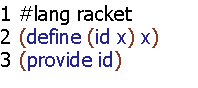
\includegraphics{figures/untyped-rkt1.pdf}
\caption{untyped1.rkt: a simple Racket file}
\label{fig:ut1r}
\end{figure}

\begin{figure}
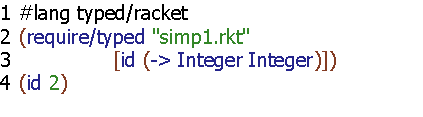
\includegraphics{figures/typed-rkt1.pdf}
\caption{typed1.rkt: Typed Racket file using untyped1.rkt}
\label{fig:t1r}
\end{figure}

This construction, whereby every module is either entirely typed or entirely
untyped allows Typed Racket to take a unique approach to enforcement, built
around contracts~\cite{tf-popl08} applied at the points where modules
interact. Types of values are checked at boundaries, and methods are
effectively wrapped as they cross between modules.

The key drawback to this approach is that a wrapper cannot establish
\emph{actual identity} the same way that \emph{concrete} type systems like
Strongscript can. Instead, wrapper or guard based systems like the Typed
Racket approach can only prove that a given untyped function will \emph{act
  like} a typed function, up to cast errors, and have to be executed every
time a value passes through a typed-untyped boundary.

As a demonstration of this, consider figure~\ref{fig:tr2}. Here we import
the same untyped function, but instead of using the correct type annotation
for the (untyped) identity function, we assert that it takes an integer and
makes it into a string. This type annotation is clearly wrong, but Typed
Racket has no way of checking that it is correct when it is applied. Rather,
we are allowed to use the \xt{id} function, and only find out that the type
is wrong when it returns a number where we expected a string.

\begin{figure}[h]
% racket format-racket.rkt ../examples/typed_racket/typed2.rkt typed-rkt2.pdf
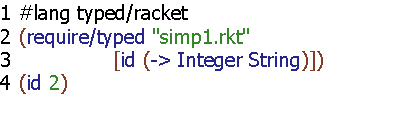
\includegraphics{figures/typed-rkt2.pdf}
\caption{typed2.rkt: Invalid type annotation}
\label{fig:tr2}
\end{figure}

However, the use of promised typing provides a major advantage: untyped code
does not need to be aware of types. In order to use a \emph{concrete} type
system, even untyped code must exist in at least an inheritance hierarchy
that can be reasoned about by the runtime type checking system. As a result,
promised typing can be used in languages that do not have class hierarchies.

While promised type systems can successfully type more code, they are
limited in that they cannot absolutely establish type correctness across
casts, unlike concrete type systems. As a result, errors occur when untyped
code is used, rather than at the boundary crossing.

\subsection{Reticulated Python}

Reticulated Python is an extension of Python adding sound gradual types by
Vitousek et al~\cite{designeval-python}, providing Python programmers with
the ability to add types to their programs. Unlike the other languages we
have examined here, though, Reticulated Python supports multiple different
semantics for these types, providing different guarantees and imposing
different restrictions.

Three different gradual typing semantics are currently avaliable in
Reticulated Python: transient, monotonic, and guarded. All three systems are
promised typing approaches, checking to ensure that untyped code behaves as
if it were typed from the perspective of a typed observer. However, the
mechanism for achieving this differs in each case.

\subsubsection{Guarded}

The guarded semantics for Reticulated Python is broadly similar to the
semantics of Typed Racket, as it uses wrappers to ensure that untyped code
behaves as expected.  However, it differs in one key area: where Typed
Racket expects typed and untyped code to be in different compilation
modules, the guarded semantics allows types to be added anywhere in the
program.

\begin{figure}[h]
\begin{verbatim}
class A1:
  def a(a : Any) : Any:
    return a + 2
class A2:
  def a(a : Int) : Int:
    return a + 2

def test(a:A2):Int
  return a.a(2) + 1

test(A1())
\end{verbatim}
\caption{Guarded: a working program.}
\label{fig:guard1}
\end{figure}

In figure~\ref{fig:guard1}, we see a correct program which runs
successfully. Class A1 is dynamically typed, and class A2 is fully
statically typed, while the test method expects a statically typed instance
of A2. We are then able to pass a dynamically typed instance of class A1
into this test method as the guarded semantics will insert a wrapper around
A1 that makes sure it acts like an A2.

To see this more clearly, we can modify the above example into
figure~\ref{fig:guard2}. Here, A1 does not act like an A2 - when passed an
argument, it will try and concatenate the string ``foo'' onto the end, and
will return a string (if it can). As a result, we know that this will
produce an error, but the question is: where?

\begin{figure}[h]
\begin{verbatim}
class A1:
  def a(a : Any) : Any:
    return a + "foo"
class A2:
  def a(a : Int) : Int:
    return a + 2

def test(a:A2):Int
  return a.a(2) + 1

test(A1())
\end{verbatim}
\caption{Guarded: A1 does not follow the types of A2, and therefore invocation fails.}
\label{fig:guard2}
\end{figure}

In this case, the error appears after the function A1.a returns, but before
the value is passed back to the caller. A wrapper is added around A1 that
checks that the return value is an instance of type int, and when it is not,
an error is produced.

The guarded semantics is one of the most intuitive of the systems we have
covered - errors are produced exactly when the value produced breaks the
type guarantee. However, it suffers from the same issues as were identified
in~\cite{practical-gt} for Typed Racket, with considerable ``wrapper
bloat'', caused when a value passes between typed and untyped code a large
number of times.

\begin{figure}[h]
\begin{verbatim}
class A1:
  def a(a : Any) : Any:
    return a + "foo"
class A2:
  def a(a : Int) : Int:
    return a + 2

def a1(a:A1):A1
  return a

def a2(a:A2):A2
  return a

a = A1()
for i=1,1000:
  a = a1(a2(a))
\end{verbatim}
\caption{Guarded: Adding a considerable number of wrappers.}
\label{fig:guard3}
\end{figure}

This problem is illustrated in figure~\ref{fig:guard3}. The functions a1 and
a2 act as casts to A1 and A2, respectively, and we apply each to the same
value 1000 times, alternating between a1 and a2. The problem here arises
from the naive interpretation of wrapping, where each time we go from A1 to
A2 we acquire a new weapper. At the end of this program, a call to a would
go through 1000 different objects!

While approaches to help simplify this particular problem exist, little
progress has been made in eliminating it entirely, at least to acceptible
levels. As a concequence, two other systems have been added in Reticulated
Python that take a different perspective on the issue of how to ensure
soundness, but at lower cost in memory and levels of indirection.

\subsubsection{Transient}

In both the Strongscript and Typed Racket approaches, if you wrote a method
(denoted $\m$ here) under type $\xt{int} \rightarrow \xt{int}$, you could be
assured that you would only ever be called with an argument that was
actually an int. To achieve this guarantee, the systems alternately
performed inline runtime casts based on runtime type information and
inserted wrappers to check that the types were respected \emph{before} an
actual function call was made. Likewise, a function that was declared to
return an int would always return an int, ensured either by wrapping or by
adding casts inside of it.

Transient takes the opposite perspective. Instead of the caller being
responsible for checking the types on the arguments and the callee ensuring
the return type is correct, the transient semantics for Reticulated Python
has the callee enforce the types on the arguments and the caller enforce the
type of the return value.

To illustrate this, consider figure~\ref{fig:guard2}. If we look at the
execution trace that produces the error, we find the following sequence of
events happened:
\begin{enumerate}
\item Evaluate \verb|A1()| to value \xt{v}
\item Wrap \xt{v} with wrapper \xt{A2W}, producing \xt{vw}
\item Invoke \verb|test| with \xt{vw}
\item Call \verb|a| with 2 on \xt{vw}
\item \xt{A2W} checks that 2 is an integer
\item Append 2 to the string ``foo'' inside \xt{A1.a}
\item Return ``2foo'' 
\item \xt{A2W} finds that ``2foo'' is not an integer, and errors.
\end{enumerate}

Likewise, in figure~\ref{fig:guard3}, we would end up with steps 5 and (a
successful) step 8 repeated 1000 times in the execution trace. However, we
can ``bake in'' the checks added by \xt{A2W} into the program itself,
resulting in figure~\ref{fig:trans1}.

\begin{figure}[h]
\begin{verbatim}
class A1:
  def a(a : Any) : Any:
    return a + "foo"
class A2:
  def a(a : Int) : Int:
    check(a, Int)
    return a + 2

def test(a:A2):Int
  return check(a.a(2), Int) + 1

test(A1())
\end{verbatim}
\caption{Transient: Type checks baked into source.}
\label{fig:trans1}
\end{figure}

This embedding preserves the execution trace that we saw in the guarded
semantics, but also completely avoids the problems inherent to having
wrappers added at type transitions. However, while the transient semantics
is able to preserve the execution trace, the site at which the error happens
is somewhat different.

In the guarded semantics, step 8 happened \emph{before} the function
\verb|a| was able to return, and therefore the caller effectively never saw
the wrong type. In the transient semantics, the caller is now responsible
for ensuring that the types of the values passed into it are correct, which
has two key implications.

The first is that the site where errors occur is now slightly
different. When a function returns a value that does not match up with the
type that it produces, that discrepancy is now noticed in the caller,
instead of inside of the wrapper.

This leads to the second implication of the transient semantics: all typed
code now has to add type checks, as seen in \verb|A2.a| in
figure~\ref{fig:trans1}. No typed code can trust any type, be that a type
that is passed in (for the case where untyped code calls typed code), or a
type returned from another function (as the other function could be
untyped).

While this approach completely avoids the problem identified in
figure~\ref{fig:guard3}, it raises a new performance issue: this check
cannot be statically removed. Any nominally typed variable can now no longer
be statically trusted to respect its type, and as a result, every invocation
must be checked for type safety. Therefore, the transient semantics will run
into performance issues, if naievly implemented, as more types are added,
contradicting the typical wisdom about types and performance. While a more
sophisticated implementation may be able to avoid some of these checks, even
better performance of typed code can be made possible by using a different
type safety guarantee.


\subsubsection{Monotonic}
A key downfall of the approaches we discussed previously is that they
cause performance impacts in fully-typed code, especially at heap access
sites.The monotonic semantics for Reticulated Python aims to recover this,
in exchange for a new dynamically-enforced guarantee.

To see why the impact exists, consider the following code

\begin{verbatim}
function evil(x : *) : * {
	x := "foo bar"
}

Ref<Int> a = Ref(3)
evil(a)
Int y = !x + 2
\end{verbatim}

If we stripped all checks from this code, we would end up with a stuck
state, since we would be adding a string to an integer, despite statically
typing the value of $\a$ as an integer, as we were able to assign to the
underlying reference from an untyped context.

The approaches discussed for Typed Racket and the transient semantics
handle this case differently, but both require that the typed code perform
a typecheck at the dereference of $\x$. Problematically, these checks
have to be performed even in a fully typed program, because it is impossible
to know which pointers have been exposed to dynamic code.

The key feature of the monotonic semantics is that it imposes these checks
on the dynamic code - any dynamic reference has to respect the types imposed
by a typed reference. In the above example, the monotonic semantics would
produce an error when we tried to assign a string into $\x$ - despite the
static typing working out, because the reference has a type which is
incompatible with our new type, monotonic will reject it at that point.
%%%%%%%%%%%%%%%%%%%%%%%%%%%%%%%%%%%%%%%%%%%%%%%%%%%%%%%%%%%%%%%%%%%%%%%%%%%

\section{Kafka: A Core Calculus}
\newcommand{\name}{{\sf KafKa}\xspace}

We propose to explore the semantics of gradually typed object-oriented
languages by compilation to a core calculus, named \name.

Following the design of C\# 4.0, \name is a statically typed class-based
calculus with dynamic dispatch.

In order to support the notion of consistency, we choose a structural type
system for \name.  The calculus does not have inheritance between classes.

\name does not have null values.\footnote{What would the type of null be?}

Fields are accessed by getter and setter methods, their presence in class
types is observed by the presence of the respective getters and setters.


Following C\#, \name allows a dynamic type, denoted \any. 

Statically dispatched method calls (i.e. calls where the type of the
receiver is not \any) are denoted \Call\x\m\e. Methods are limited to a
single argument for simplicity.

Dynamically dispatched method calls (i.e. call where the type of the receiver
is \any) are denoted \DynCall\x\m\e.

A new object is created with a class name and a sequence of arguments in the
order of definition of fields, denoted \New\C{\b\e}.

Meta-variable \x ranges over argument names, \a over memory locations, \f
over field names (as well as getter and setter methods), \m over method
names, \C, \D, and \E over class names.  We use \n to refer either to
methods or field names.

\this is a distinguished variable name that denotes the current object.

\that is a distinguished field name that denotes the target of a wrapper.

\D is a meta-variable used to range over dynamically generated class names.

\a is ranges over heap addresses.

\k ranges over class definitions consisting of a class name, followed by
a, possibly empty, sequence of field definitions, \fd, and a, possibly empty,
sequence of method definitions, \md.

\begin{figure}[!h]
\hrulefill

\begin{minipage}{6.3cm}\begin{tabular}{@{}l@{~}l@{}l@{}l@{}ll}
\e &::=  \x         &\B \this         &\B \that        &\B \New\C{\b\e} \\
   &\B \Get\e\f     &\B \Set\e\f\e    &\B \Call\e\m\e  &\B \DynCall\e\m\e \\
   &\B \SubCast\t\e &\B \ShaCast\t\e  &\B \BehCast\t\e &\B  \MonCast\t\e \\
   &\B \a \\ 
\end{tabular}\end{minipage}
\begin{minipage}{6cm}\begin{tabular}{l@{~}l@{}l@{}l}
   ~ \k &::= \Class \C {\b\fd}{\b\md}
\end{tabular}
\begin{tabular}{l@{~}l@{}l@{}l}
\md &::= \Mdef\m\x\t\t\e   &\B  \Mdef\f\x\t\t\e &\B \Mdefz\f\t\e \\
\mt &::= \Mtype\m\t\t &\B~  \Mtype\f\t\t  &\B \Mtype\f{}\t  \\
~ \t&::= ~ \any  \B   \C  & \fd~ ::= ~ \Fdef\f\t \\ 
\end{tabular}\end{minipage}

\hrulefill

\caption{\name Syntax.}\label{syn}
\end{figure}

%% TODO Put somewhere????
%\E  &::= \Ftype\x\t  \B \none\\
% \s  &::= ~~\none ~~ \B ~~  {\Bind{\a}{\obj\C{\b\a}}}~\s


\name has four different kinds of cast expressions, two are structural and
two are generative. The structural subtype cast, denoted \SubCast\t\a,
asserts that the object at location \a is of type \t.  The structural
shallow cast, denoted \ShaCast\t\a, asserts that the object at location \a
has methods with names matching those of \t. This does not make any
guarantee about the type of arguments.  The generative behavioral cast,
denoted \BehCast\t\a, will ensure that either \a behaves as a \t or that it
get stuck. The generative monotonic cast, denoted \MonCast\t\a, is a
behavioral cast that, in addition, imposes constraints on fields.


\subsection{Semantics}

The semantics of \name is defined by a small step operational semantics with
evaluation contexts.

Evaluation context deterministically identifiy the next expression to evaluate.

Program error is denoted by a stuck term.

The semantics operate over an explicit class table, denoted \K, which is a
sequence of class definitions.

A heap, denoted \s, maps memory locations to
objects. We use the notation \Heap\s{\Bind\a{\obj\C{\b\a}}} to denote the
heap \s extended by the binding of location \a to object \obj\C{\b\a}.

A configuration \K\e\s evaluates in one step to a new configuration, denoted
\Reduce \K\e\s \Kp\ep\sp.

Execution terminate if \ep\xspace is a value, \a, or if there is no applicable
reduction, in which case the program is stuck.\footnote{Intuitively we would
  expect that the program can only get stuck at dynamic calls or at
  structural casts. But generative casts add some complexity to that
  statement.}

New object creation picks a fresh memory location  and binds it to the
newly created.

Operations on fields require a typed receiver, for example in the expression
\Get\this\f, \this is always of the type of the current class. Field access
through a getter method, works as follows. If the receiver's class has a
getter method, that method is evaluated, otherwise the field corresponding
the getter's name is updated.

Methods are segregated into typed method (methods whose argument is not
\any) and untyped method (methods whose argument is \any). The former can be
called by statically resolved method, the latter must be called by
dynamically resolved methods.

The function \names{} returns the names of methods. 

The function \untyped{} returns the methods whose types are \any.

The auxiliary function \xt{read} return the location \ap pointing to the
field \f of the object at location \a. The auxiliary function \xt{write}
return the heap \sp with the field \f of the object at location \a updated
to the location \ap.

We write \App\K\C to denote the lookup of class \C in class table \K.

We write  \Mdef\m\x\t\tp\e \In \k to denote that method \m occurs in class \k.

Ordering within lists of fields and methods definition is not relevant. (ie we can reorder when convenient)


\begin{figure}[!h]
\hrulefill

\begin{minipage}{8cm}
  \opdef{\Reduce \K\e\s \Kp\ep\sp}
        {\e\s evaluates to \ep\xspace in a step}\\[-1mm]
\begin{tabular}{l@{}l@{~}l@{~}l}
\CondRule{E1}{  %% new C -> a
   \ap fresh
}{ 
  \ReduceA \K{\New\C{\b\a}}\s \K\ap{\Heap\s{\Bind\ap{\obj\C{\b\a}}}}
}
\CondRule{E2}{  %% a.f() -> e
    \Mdefz\f\t\e \In \App\K\C \AND \obj\C{\b\a} = \App\s\a
}{
   \ReduceA \K{\Get\a\f}\s \K{[\a/\this]\e}\s
}
\CondRule{E3}{  %% a.f(a) -> e
    \Mdef\f\x\t\t\e \In \App\K\C \AND \obj\C{\b\a} = \App\s\a
}{
   \ReduceA \K{\Set\a\f\ap}\s \K{[\a/\this~{\ap/\x}]\e}\s
}
\CondRule{E4}{  %% a.f() -> e
 \ap = \readf \s\a\f\K
}{
  \ReduceA \K{\Get\a{\f}}\s  \K\ap\s
}
\CondRule{E5}{  %% a.f(e) -> e
 \sp = \setf \s\a\f\ap\K
}{
  \ReduceA \K{\Set\a{\f}\ap}\s \K\ap\sp
}
\CondRule{E6}{  %% a.m(a) -> e
  \Mdef\m\x\D\Dp\e  \In \App\K\C \AND \obj\C{\b\a} = \App\s\a 
}{
 \ReduceA \K{\Call\a\m\ap}\s \K{[\a/\this~{\ap/\x}]\e}\s
}
\CondRule{E7}{  %% a@m(a) -> e
    \Mdef\m\x\any\any\e \In \App\K\C \AND \obj\C{\b\a} = \App\s\a
}{
  \ReduceA \K{\DynCall\a\m\ap}\s \K{[\a/\this~{\ap/\x}]\e}\s
}
\CondRule{E8}{  %% Subtypecast
}{ 
  \ReduceA \K{\SubCast \any\a}\s \K\a\s
}
\CondRule{E9}{  %% Subtypecast
  \StrSub {}\K\C \D \AND \obj\C{\b\a} = \App\s\a
}{ 
  \ReduceA \K{\SubCast \D\a}\s \K\a\s
}
\CondRule{E10}{  %% Shallow Structural
}{ 
  \ReduceA \K{\ShaCast \any\a}\s \K\a\s
}
\CondRule{E10b}{  %% Shallow Structural
 \names{\untyped{\App\K\C}}  $\supseteq$  \names{\untyped{\App\K\D}} \AND \obj\C{\b\a} = \App\s\a
}{ 
  \ReduceA \K{\ShaCast \D\a}\s \K\a\s
}
\CondRule{E11}{  %% Behavioral cast
  \behcast \a\t\s\K  \Kp\ap\sp
}{ 
  \ReduceA  \K{\BehCast \t\a}\s \Kp\ap\sp
}
\CondRule{E12}{  %% Monotonic cast
  \moncast \a\t\s\K  \Kp\sp
}{ 
  \ReduceA \K{\MonCast\t\a}\s \Kp\a\sp
}
\CondRule{E13}{  %% E[e] -> E[e']
  \Reduce \K\e\s \Kp\ep\sp
}{
 \ReduceA \K{\EE[\e]}\s \Kp{\EE[\ep]}\sp
}
\end{tabular}\end{minipage}

%%%%%%%%%%%%%%%%%%% CONTEXTS %%%%%%%%%%%%%%%%%%%%%%%%%%%%%%%%%%%%%%%%%%%%
~\\[2mm]

\begin{minipage}{4cm}\begin{tabular}{l@{~~}l@{~}l@{~}l@{~}l@{~}l@{~}l@{~}l}
\EE &::= \Get\EE\f     &\B
        \Set\EE\f\e   &\B
        \Set\a\f\EE   &\B  
        \Call\EE\m\e  &\B
        \Call\a\m{\EE} &\B
        \DynCall\EE\m\e   &\B
        \DynCall\a\m\EE   \\
   &\B~
       \SubCast\t\EE  &\B
       \ShaCast\t\EE  &\B
       \BehCast\t\EE &\B
       \MonCast\t\EE  &\B
       \New\C{\b \a\,\EE\,\b\e}
  &\B \EM{\square}
\end{tabular}
\end{minipage}

\hrulefill
\caption{\name Semantics.}
\end{figure}


\section{Translations}

KafKa provides us with a basis through which we can describe the operation of more typical languages. KafKa requires that the programmer write casts wherever a type boundary is encountered, which is not representative of how actual gradually typed programming languages behave. Most gradually typed programming languages abstract away from the actual casts that are inserted, automatically inserting them and using them at runtime, invisibly to the programmer up until it produces an error.

To represent this, we introduce a \emph{translation} mechanism, that performs much the same duty that this step does. This step works very similarly to how Siek and Taha~\cite{SiekTaha06} described cast insertion, though, thanks to our more complex source and target languages, we cannot entirely use the simple, bottom-up approach that Siek and Taha did.

Instead, we use a \emph{bidirectional} translation mechanism, based on the work originally done by Pierce and Turner~\cite{lti-pierce}. Bidirectional typechecking is, in effect, a local type inference mechanism, and allows us to cleanly identify cast insertion locations in a modular way.

\newcommand{\progtrans}[2]{#1 ~\hookrightarrow_p~ #2}
\newcommand{\classtrans}[3]{#1 \vdash #2 ~\hookrightarrow_c~ #3}
\newcommand{\methtrans}[3]{#1 \vdash #2 ~\hookrightarrow_m~ #3}
\begin{mathpar}
\IRule{PT}{
  {\classtrans{\K}{\K}{\K'}} \\ \GenCast{\K}{\cdot}{\e}{\ep}{\t} 
}{\progtrans{\e~\K}{\e'~{\K'}}}

\IRule{CR1}{ 
  \b{\methtrans{\K}{\md}{\md'}} \\
  \classtrans{\K}{\K'}{\K''}
}{\classtrans{\K}{\Class \C {\b{\Ftype\f\t}}{\b\md}~\K'}{\Class \C {\b{\Ftype\f\t}}{\b{\md'}}~\K''}}

\IRule{CR2}{ }{\classtrans{\K}{\cdot}{\cdot}}

\IRule{MT}{
  \AnaCast{\K}{\HT\x\t}{\e}{\ep}{\tp}
}{\methtrans\K{\Mdef\m\x\t\tp\e}{\Mdef\m\x\t\tp\ep}}
\end{mathpar}

\subsection{Strongscript}

\newcommand{\bC}{\xt{!C}}

\begin{tabular}{l@{~~}l@{}l@{}l}
\t  &::= ~ \any \B \C \B \bC \\ 
\end{tabular}

\newcommand{\ba}{\xt{!}}
\begin{mathpar}
\IRule{A1}{\HasType{\E}\x\t}{\GenCast{\K}\E\x\x\t}

\IRule[width=30em]{A2}{
    \GenCast{\K}{\E}{\e_1}{\e_3}{\bC} \\ \n(\b{\t_1}):\t_2 \in \classoff\C\K \\ \b{\AnaCast{\K}{\E}{\e_2}{\e_4}{\t_1}}
}{
    \GenCast{\K}{\E}{\Call{\e_1}\n{\b{\e_2}}}{\Call{\e_3}\n{\b{\e_4}}}{\t_2}
}

\IRule{A5}{
    \GenCast{\K}{\E}{\e_1}{\e_3}{\C} \\ \m({\t_1}):\ba\D \in \classoff\C\K \\ {\AnaCast{\K}{\E}{\e_2}{\e_4}{\t_1}} 
}{
    \GenCast{\K}{\E}{\Call{\e_1}\m{{\e_2}}}{\SubCast{\D}{\DynCall{\e_3}\m{{\e_4}}}}{\bC} %Q: do I need to cast the return value of non-bang
}

\IRule{A6}{
    \GenCast{\K}{\E}{\e_1}{\e_3}{\C} \\ \m({\t_1}):\t_2 \in \classoff\C\K \\ \t_2 \neq \ba\D \\ {\AnaCast{\K}{\E}{\e_2}{\e_4}{\t_1} }
}{
    \GenCast{\K}{\E}{\Call{\e_1}\m{{\e_2}}}{\DynCall{\e_3}\m{{\e_4}}}{\C} %Q: do I need to cast the return value of non-bang
}

\IRule{A8}{
    \GenCast{\K}{\E}{\e_1}{\e_3}{\any} \\ {\AnaCast{\K}{\E}{\e_2}{\e_4}{\any}}
}{
    \GenCast{\K}{\E}{\Call{\e_1}\m{{\e_2}}}{\DynCall{\e_3}\m{{\e_4}}}{\any}
}

\IRule{A11}{
  \b{\AnaCast{\K}\E{\e_1}{\e_2}\t} \\ 
  \Class \C {\b{\Ftype\f\t}} {\b{\md}}
  }{\GenCast{\K}{\E}{\New\C{\b{\e_1}}}{\New\C{\b{\e_2}}}{\C}}
\end{mathpar}

\hrulefill

\begin{mathpar}
\IRule{AASC1}{
  \GenCast{\K}{\E}{\e_1}{\e_2}{\bC_2} \\
  {\C_2}\Sub{\C_1}\\
}{
  \AnaCast{\K}{\E}{\e_1}{\e_2}{\bC_1}
}

\IRule{AASC2}{
  \GenCast{\K}{\E}{\e_1}{\e_2}{\bC_2} \\
  \K \vdash {\C_2}\Sub{\C_1}\\
}{
  \AnaCast{\K}{\E}{\e_1}{\e_2}{\C_1}
}

\IRule{AASC3}{
  \GenCast{\K}{\E}{\e_1}{\e_2}{\C_2} \\
  {\C_2}\Sub{\C_1}\\
}{
  \AnaCast{\K}{\E}{\e_1}{\e_2}{\C_1}
}

\IRule{AASC4}{
  \GenCast{\K}{\E}{\e_1}{\e_2}{\C} \\
}{
  \AnaCast{\K}{\E}{\e_1}{\SubCast{\C}{\e_2}}{\bC}
}

\IRule{AASC5}{
  \GenCast{\K}{\E}{\e_1}{\e_2}{\any} \\
}{
  \AnaCast{\K}{\E}{\e_1}{\SubCast{\C}{\e_2}}{\bC}
}

\IRule{AASC6}{
  \GenCast{\K}{\E}{\e_1}{\e_2}{\any} \\
}{
  \AnaCast{\K}{\E}{\e_1}{\e_2}{\C}
}

\IRule{AASC7}{
  \GenCast{\K}{\E}{\e_1}{\e_2}{\t} \\ \t \neq \any
}{
  \AnaCast{\K}{\E}{\e_1}{\e_2}{\any}
}
\end{mathpar}

\subsection{Typed Racket}

The Typed Racket formalism we present is not strictly limited to the Typed Racket language - as in that case, we would be modelling a normal typed object calculus, and not a gradual type system.

As a result, we present the interaction between modules written in both Typed Racket and Racket. Notably, we do not represent the limitation that typed code can only exist in one language and untyped code in the other, as it does not have a considerable impact on the semantics of the language, at least at the level we are considering.

\begin{mathpar}
\IRule{A1}{\HasType{\E}\x\t}{\GenCast{\K}\E\x\x\t}

\IRule[width=30em]{A2}{
    \GenCast{\K}{\E}{\e_1}{\e_3}{\C} \\ \n(\b{\t_1}):\t_2 \in \classoff\C\K \\ \b{\AnaCast{\K}{\E}{\e_2}{\e_4}{\t_1}}
}{
    \GenCast{\K}{\E}{\Call{\e_1}\n{\b{\e_2}}}{\Call{\e_3}\n{\b{\e_4}}}{\t_2}
}

\IRule{A8}{
    \GenCast{\K}{\E}{\e_1}{\e_3}{\any} \\ {\AnaCast{\K}{\E}{\e_2}{\e_4}{\any}}
}{
    \GenCast{\K}{\E}{\Call{\e_1}\m{{\e_2}}}{\DynCall{\e_3}\m{{\e_4}}}{\any}
}

\IRule{A11}{
  \b{\AnaCast{\K}\E{\e_1}{\e_2}\t} \\ 
  \Class \C {\b{\Ftype\f\t}} {\b{\md}}
  }{\GenCast{\K}{\E}{\New\C{\b{\e_1}}}{\New\C{\b{\e_2}}}{\C}}
\end{mathpar}

Typed Racket uses the simplest translation, as it does not introduce any new types, and relies entirely on wrappers to ensure correctness. As a result, we can use just two rules for calling - one for typed, the other for typed - and the rest of the cases simply reduce trivially.

\begin{mathpar}
\IRule{AASC1}{
  \GenCast\K\E\e\ep\tp \\
  \K \vdash \tp \Sub \t
}{
  \AnaCast\K\E\e\ep\t
}

\IRule{AASC2}{
  \GenCast\K\E\e\ep\tp
}{
  \AnaCast\K\E\e{\BehCast\t\ep}\t
}
\end{mathpar}

Likewise, as Typed Racket imposes no restrictions on what is technically possible to assert types on, we do not either. If the system cannot statically show compatibility, then it will wrap whatever it encountered to ensure that its behaviour is correct, then pass it on.

\subsection{Reticulated Python}

Reticulated Python is somewhat more complicated, as it implements three different semantics, though not simultaneously. As a result, we will show translations for each of its three semantics options.

The most notable difference between Reticulated and the other systems at the surface level is the use of \emph{consistency}, an operator broadly meaning that one type is compatible with another type. In our system, we define conistency as follows:
\newcommand{\consistent}[3]{#1 \vdash #2 ~\sim~ #3}
\begin{mathpar}
\IRule{C1}{\meett{\cdot, \K, \C, \D} = \t~{\K'}}{\consistent\K{\C}{\D}}
\end{mathpar}

In effect, if there is some most specific type for two given types, then the two types are consistent - it is possible that a value of one could be converted into the other with a runtime cast.

\paragraph{Guarded}

The guarded semantics for Reticulated Python is essentially identical to the semantics we propose for Typed Racket, where values are converted from typed to untyped by wrappers applied over boundaries. The only notable difference in our context is that the guarded semantics uses consistency to ensure that the types are actually convertible, whereas the Typed Racket system will always allow values to pass.


\begin{mathpar}
\IRule{A1}{\HasType{\E}\x\t}{\GenCast{\K}\E\x\x\t}

\IRule[width=30em]{A2}{
    \GenCast{\K}{\E}{\e_1}{\e_3}{\C} \\ \n(\b{\t_1}):\t_2 \in \classoff\C\K \\ \b{\AnaCast{\K}{\E}{\e_2}{\e_4}{\t_1}}
}{
    \GenCast{\K}{\E}{\Call{\e_1}\n{\b{\e_2}}}{\Call{\e_3}\n{\b{\e_4}}}{\t_2}
}

\IRule{A8}{
    \GenCast{\K}{\E}{\e_1}{\e_3}{\any} \\ {\AnaCast{\K}{\E}{\e_2}{\e_4}{\any}}
}{
    \GenCast{\K}{\E}{\Call{\e_1}\m{{\e_2}}}{\DynCall{\e_3}\m{{\e_4}}}{\any}
}

\IRule{A11}{
  \b{\AnaCast{\K}\E{\e_1}{\e_2}\t} \\ 
  \Class \C {\b{\Ftype\f\t}} {\b{\md}}
  }{\GenCast{\K}{\E}{\New\C{\b{\e_1}}}{\New\C{\b{\e_2}}}{\C}}
\end{mathpar}

\begin{mathpar}
\IRule{AASC1}{
  \GenCast\K\E\e\ep\tp \\
  \K \vdash \tp \Sub \t
}{
  \AnaCast\K\E\e\ep\t
}

\IRule{AASC2}{
  \GenCast\K\E\e\ep\tp \\
  \consistent\K\t\tp
}{
  \AnaCast\K\E\e{\BehCast\t\ep}\t
}
\end{mathpar}


\paragraph{Transient}

The transient semantics is notably different from the other systems, as illustrated by the invariants we can assume about its primary cast, $\ShaCast\t\e$. Here, we simply assert that $\e$ has the same \emph{names} as $\t$ does, and, as a result, the closest type representation we have is the $\any$ type, as illustrated in the typing for KafKa. All Transient guarantees is that the methods on the named type will be callable with some argument, and some return value, and it is up to the callee to check that the arguments are right and up to the caller to ensure that the return value is right.

Because of fields, we cannot fully represent the transient semantics in KafKa, as field accessors and getters can only be called in a fully typed context. However, we can approximate it, by only allowing field getters and setters to be called in the context of \this, thereby removing all possible ambiguity over the receiver of the field getter or setter.


\begin{mathpar}
\IRule{MTU}{
  \AnaCast{\K}{\HT\x\any}{\e}{\ep}{\any}
}{\methtrans\K{\Mdef\m\x\any\any\e}{\Mdef\m\x\any\any\ep}}

\IRule{MTT}{
  \t \neq \any \\
  \AnaCast{\K}{\HT\x\t}{\e}{\ep}{\tp}
}{\methtrans\K{\Mdef\m\x\t\tp\e}{\Mdef\m\x\any\any{\SubCast{\any}{\New{\EMxt A2}{\ShaCast\t\x, \e}.f2()}}}}
\end{mathpar}


\begin{mathpar}
\IRule{A1}{\HasType{\E}\x\t}{\GenCast{\K}\E\x{\ShaCast\t\x}\t}

\IRule[width=30em]{A2}{
    \GenCast{\K}{\E}{\e_1}{\e_3}{\C} \\ \n(\b{\t_1}):\t_2 \in \classoff\C\K \\ \b{\AnaCast{\K}{\E}{\e_2}{\e_4}{\t_1}}
}{
    \GenCast{\K}{\E}{\Call{\e_1}\n{\b{\e_2}}}{\ShaCast{\t_2}{\Call{\e_3}\n{\b{\e_4}}}}     {\t_2}
}

\IRule{A8}{
    \GenCast{\K}{\E}{\e_1}{\e_3}{\any} \\ {\AnaCast{\K}{\E}{\e_2}{\e_4}{\any}}
}{
    \GenCast{\K}{\E}{\Call{\e_1}\m{{\e_2}}}{\DynCall{\e_3}\m{{\e_4}}}{\any}
}

\IRule{A11}{
  \b{\AnaCast{\K}\E{\e_1}{\e_2}\t} \\ 
  \Class \C {\b{\Ftype\f\t}} {\b{\md}}
  }{\GenCast{\K}{\E}{\New\C{\b{\e_1}}}{\New\C{\b{\e_2}}}{\C}}
\end{mathpar}

\begin{mathpar}
\IRule{AASC1}{
  \GenCast\K\E\e\ep\tp \\
  \K \vdash \tp \Sub \t
}{
  \AnaCast\K\E\e\ep\t
}

\IRule{AASC2}{
  \GenCast\K\E\e\ep\tp \\
  \consistent\K\tp\t
}{
  \AnaCast\K\E\e\ep\t
}
\end{mathpar}

\paragraph{Monotonic}


\bibliographystyle{plain}
\bibliography{../bib/compactdoi}

\appendix
%%%%%%%%%%%%%%%%%%%%%%%%%%%%%%%%%%%%%%%%%%%%%%%%%%%%%%%%%%%%%%%%%%%%%%%%%%%%%%
%%%%%%%%%%%%%%%%%%%%%%%%%%%%%%%%%%%%%%%%%%%%%%%%%%%%%%%%%%%%%%%%%%%%%%%%%%%%%%
%%%%%%%%%%%%%%%%%%%%%%%%%%%%%%%%%%
%%%%%%%%%%%%%%%%%%%%%%%%%%%%%%%%%%%%%%%%%%%%%%%%%%%%%%%%%%%%%%%%%%%%%%%%%%%
\section{Auxiliary Definitions}%%%%%%%%%%%%%%%%%%%%%%%%%%%%%%%%%%%%%%%%%%%%%%%
%%%%%%%%%%%%%%%%%%%%%%%%%%%%%%%%%%%%%%%%%%%%%%%%%%%%%%%%%%%%%%%%%%%%%%%%%%%%%%
%%%%%%%%%%%%%%%%%%%%%%%%%%%%%%%%%%%%%%%%%%%%%%%%%%%%%%%%%%%%%%%%%%%%%%%%%%%%%%

\subsection{Subtyping}

The structural subtype relation, written \StrSub\M\K\t\tp, asserts that \t
is a subtype of \tp in the environment composed of a set of subtyping \M and
a class table \K.   The set of subtypings can be omitted if empty.

~\\

\opdef{\StrSub\M\K\t\tp}{\t is a subtype of \tp}
\begin{mathpar}
\IRule{SRef}{
}{
 \StrSub\M\K \t \t
}

\IRule{SAss}{
\C \Sub \D \in \M
}{
 \StrSub \M\K \C \D
}

\IRule{SRec}{
 \Class\D{\b\fd}{\b\md}\in\K\\
 \M' = \M~\C\Sub\D\\
 \fd\in\b\fd \implies \StrSub{\M'}\K \C \fd\\
 \md\in\b\md \implies \StrSub{\M'}\K \C \md\\
}{
 \StrSub \M\K \C \D 
}
\end{mathpar}

Several auxiliary rules are used in the subtype judgement. 

\begin{mathpar}
\IRule{SMet}{
  \Mdef\m\x{\t_2}{\t_2'}\e\In\App\K\C \\
  \StrSub \M\K \t {\t_2} \\
  \StrSub \M\K {\t_2'} \tp
}{
 \StrSub \M\K \C {\Mdef\m\x\t\tp\e}
}

\IRule{SFie}{
  \Fdef\f\t\In\App\K\C
}{
 \StrSub \M\K \C {\Fdef\f\t}
}

\IRule{SSet}{
  \Fdef\f\t\In\App\K\C
}{
 \StrSub \M\K \C {\Mdef\f\x\t\t\e}
}

\IRule{SGet}{
  \Fdef\f\t\In\App\K\C
}{
 \StrSub \M\K \C {\Mdefz\f\t\e}
}
\end{mathpar}

\subsection{Well-formedness}

The overloading function is meant to check that every typed method is
defined once. Every untyped method is defined once. A class has either a
field \f or a pair of getter and setters.

\opdef{\WF{}\s\K {\Class\C{\b\fd}{\b\md}}}{Well-formed class}

\begin{mathpar}
\IRule{WC}{
 \xt{overloading}(\b\fd,\b\md)\OK \\
 \fd\in\b\fd\implies \WF \none\s\K \fd \\
 \md\in\b\md\implies \WF \none\s\K \md 
}{
 \WF {}\s\K {\Class \C {\b\fd}{\b\md}}
}
\end{mathpar}

We have some auxiliary judgements.

\begin{mathpar}
\IRule[width=18em]{WT}{
 \EnvType {\E{\Ftype\x\C}}\s\K\e\D\\
 \WFtype\K\C \\
 \WFtype\K\D \\
}{
 \WF \E\s\K {\Mdef\m\x\C\D\e}
}

\IRule[width=18em]{WU}{
 \EnvType {\E \Ftype\x\any}\s\K \e\any\\
}{
 \WF \E\s\K{\Mdef\m\x\any\any\e}
}

\IRule{WS}{
 \EnvType {\E{\Ftype\x\tp}}\s\K \e\t \\
 \WFtype \K\t 
}{
 \WF  \E\s\K {\Mdef\f\x\t\t\e}
}

\IRule{WF}{
 \WFtype \K\t 
}{
 \WF  \E\s\K {\Fdef\f\t}
}

\IRule{WG}{
 \EnvType \E\s\K\e\t \\
 \WFtype \K\t
}{
 \WF \E\s\K {\Mdefz\f\t\e}
}


\IRule{WA}{
}{
 \WFtype \K \any
}

\IRule{WC}{
 \C \in \K
}{
 \WFtype  \K\C
}
\end{mathpar}



\subsection{Typing}



Type checking is standard.

Field accessor rules W3 and W4 require a typed receiver, since \any does
not have any methods a receiver typed at \any will never typecheck.

Shallow casts, W9, do not change the type of the expression. We are casting
to the name of \t not to \t.  In practice that means that all expression
types in Transient will drift towards \any.

~\\

\opdef{\EnvType\E\s\K\e\t}{\e has type \t in environment \E against heap \s}
\begin{mathpar}

\IRule{W1}{
   \HasType \E\x\t
 }{
   \EnvType \E\s\K\x\t
}

\IRule{W2}{
  \EnvType \E\s\K\e\tp \\
 \StrSub \M\K \tp \t
 }{
  \EnvType \E\s\K\e\t 
}   

\IRule{W3}{
  \EnvType \E\s\K\e\C \\
  \Mtype \f{}\tp \in \K(\C)
}{
  \EnvType \E\s\K{\Get\e\f}\tp
}    

\IRule{W4}{
  \EnvType \E\s\K\e\C \\
  \Mtype \f\tp\tp \in \K(\C)  \\
  \EnvType \E\s\K\ep\tp
}{
  \EnvType \E\s\K{\Set\e\f\ep}\tp
}    

\IRule{W5}{
  \EnvType \E\s\K\e\C \\
  \Mtype \m\tp\tpp\in \K(\C)  \\
  \EnvType \E\s\K\ep\tp
}{
  \EnvType \E\s\K{\Call\e\m\ep}\tpp
}    

\IRule{W6}{
  \EnvType \E\s\K\e\any \\
  \EnvType \E\s\K\ep\any
}{
  \EnvType \E\s\K{\DynCall\e\m\ep}\any
}    

\IRule{W7}{
 \EnvType \E\s\K{\e_1}{\t_1}\dots 
 \EnvType \E\s\K{\e_n}{\t_n}\ \\ 
 \b\fd=\Fdef{\f_1}{\t_1}\dots\Fdef{\f_n}{\t_n} \\ 
  \Class \C {\b\fd}{\b\md} \in \K
}{
  \EnvType \E\s\K{\New\C{\e_1\dots\e_n}}\C
}

\IRule{W8}{
  \EnvType \E\s\K\e\tp
}{
  \EnvType \E\s\K{\SubCast\t\e}\t
}

\IRule{W9}{
  \EnvType \E\s\K\e\tp
}{
  \EnvType \E\s\K{\ShaCast\t\e}\any  %%!!!  not \t !!!
}

\IRule{W10}{
  \EnvType \E\s\K\e\tp
}{
  \EnvType \E\s\K{\BehCast\t\e}\t
}

\IRule{W11}{
  \EnvType \E\s\K\e\tp
}{
  \EnvType \E\s\K{\MonCast\t\e}\t
}

\IRule{W12}{
  \s(\a) = \obj\C{\b\ap}
}{
  \EnvType \E\s\K\a\C
}
\end{mathpar}


\subsection{Field read}

We write \readf\s\a\f\K to denote a read of field \f from the object
stored at \a in \s.

\begin{equation*}
\readf \s\a\f\K = \ap ~~\mathit{if}~~  \s(\a) = \obj\C{\a_1\dots\a_n \ap \dots} \AND
 \Class\C {\Fdef{\f_1}{\t_1}\dots\Fdef{\f_n}{\t_n}\Ftype\f\t\dots}{\b\md}\in\K
\end{equation*}

\subsection{Write field}

We write \setf\s\a\f\ap\K to denote the write of value \ap into field \f of
the object stored at \a in \s.

\begin{equation*}
\setf \s\a\f\ap\K= \Heap\s{\Bind{\a}{\obj\C{\a_1\dots\a_n\,\ap\dots}}}
  ~~\mathit{if}~~ \begin{cases}
   \s(\a) = \obj\C{\a_1\dots\a_n\,\app\dots}\\
   \Class\C{\Fdef{\f_1}{\t_1}\dots\Fdef{\f_n}{\t_n}\,\Fdef\f\t\dots}{\b\md}\in\K
\end{cases}
\end{equation*}




\subsection{others}

%TODO Fix ME \mtype\m\C\K = \convert{\methz\m\C\K} 

\hrulefill

\opdef{\classoff\C\K}{Auxiliary function: Type definition}

\begin{equation*}
\classoff\C\K = \EMxt{MT} ~~s.t.~~ \begin{cases}

 \K(\C) = \Class \C {\b{\Ftype\f\t}}{\b\md} \\
 \EMxt{MT} = \{\convert{\b\md} \oplus \forall ~\Ftype\fp\tp \in \b{\Ftype\f\t} ~|~ \fp \notin \b{\names{\md}} ~.~ \convertFD{\Ftype\fp\tp}\}

\end{cases}
\end{equation*}

\hrulefill


\opdef{\classoffs\a\s\K}{Auxiliary function: Type definition}

\begin{equation*}
\classoffs\a\s\K = \EMxt{MT} ~~s.t.~~ \begin{cases}

 \s(\a) = \obj\C{\b\a} \\
 \K(\C) = \Class \C {\b{\Ftype\f\t}}{\b\md} \\
 \EMxt{MT} = \{\convert{\b\md} \oplus \forall ~\Ftype\fp\tp \in \b{\Ftype\f\t} ~|~ \fp \notin \b{\names{\md}} ~.~ \convertFD{\Ftype\fp\tp}\}

\end{cases}
\end{equation*}

\hrulefill

\opdef{\ftype\f\C\K}{Auxiliary function: Field type lookup}

\begin{equation*}
\ftype\f\C\K = \t ~~s.t.~~ \begin{cases}

 \K(\C) = \Class \C {\ldots ~ \Ftype\f\t ~ \ldots}{\b\md}
\end{cases}
\end{equation*}

\hrulefill

\opdef{\field\C\K}{Auxiliary function: Field definition}

\begin{equation*}
\field\C\K = \b{\Ftype\f\t} ~~s.t.~~ \begin{cases}

 \K(\C) = \Class \C {\b{\Ftype\f\t}}{\b\md}
\end{cases}
\end{equation*}





\end{document}

%######## ##    ## ########      #######  ########    ########   #######   ######  ##     ## ##     ## ######## ##    ## ######## 
%##       ###   ## ##     ##    ##     ## ##          ##     ## ##     ## ##    ## ##     ## ###   ### ##       ###   ##    ##    
%##       ####  ## ##     ##    ##     ## ##          ##     ## ##     ## ##       ##     ## #### #### ##       ####  ##    ##    
%######   ## ## ## ##     ##    ##     ## ######      ##     ## ##     ## ##       ##     ## ## ### ## ######   ## ## ##    ##    
%##       ##  #### ##     ##    ##     ## ##          ##     ## ##     ## ##       ##     ## ##     ## ##       ##  ####    ##    
%##       ##   ### ##     ##    ##     ## ##          ##     ## ##     ## ##    ## ##     ## ##     ## ##       ##   ###    ##    
%######## ##    ## ########      #######  ##          ########   #######   ######   #######  ##     ## ######## ##    ##    ##    



This common core is focused on the basics of object functionality, with a
simple example being a \xt{Point} class.\footnote{For our examples we use
  integers and common arithmetic operations even if they are not in core
  calculus.}

%%% FIXME: formatting
\begin{verbatim}
class Point {
  x : Int
  y : Int
  addx( v : Int ) : Int {
       this.x!( this.x() + v )
  }
  addy( v : Int ) : Int {
       this.y!( this.y() + v )
  }
}
\end{verbatim}

The type system ensures that, if \xt{pt} is declared to be of type
\xt{Point}, an operation such as \xt{pt.addx(42)} will not get stuck.  As
this small language requires all variables to be initialized, there checking
for \xt{null} is not needed as it likely would in a full fledged language.

The language also supports a single unconstrained type, denote \any (pronounced
dyn), thus one could write the following method

%%% FIXME: formatting
\begin{verbatim}
  mkPt( u : * ) : Point {
      new Point( u.x() 
                 (<Point> u).y() )
  }
\end{verbatim}

This method will accept an instance of any class and will return a new
\xt{Point}. At run-time, the code will get stuck if the dynamic cast
\xt{\Cast{\xt{Point}}{\xt{u}}} fails. If \x is a declared of type \any, an
expression such as \xt{u.x()} will fail if the object bound to \xt{u} does
not have a getter \xt{x()}.


%%%%%%%%%%%%%%%%%%%%%% DYNAMIC SEMANTICS %%%%%%%%%%%%%%%%%%%%%%%%%%%%%%%%%%%%%%

The dynamic semantics evaluates expression extended with object references,
denoted \a, and errors, denoted \err, together with a heap \s mapping
references to object values. Object values contain all fields, methods, a
type, and a class; they are denoted \Obj{\b\a}\C. The class is used for
locating methods and the type is used for type casts. The need for keeping
them separate will become clear later.

The semantics uses evaluation context \E[\e], meaning that $\e$ is in the 
hole of $\E$. Selecting an object from the heap is written \Sel\s\a, 
while a heap is extended with a new object by \Heap{\s}{\Bind{\a}{\Obj{\dots}\C}}.

For an object reference \a, such that \EM{\Sel\s\a=\Obj{\dots}\C}, we have 
\classofis{\Sel\s\a}\C and \typeofis\s\a\t.

We use the notation \Mdef\m\x\t\t \inc\C to select a method in a class
definition and \Fdef\f\t\a\inc\Obj{\dots}\C to express the selection of a
field. Lastly a field of an object can be update with the notation
\Update{\Obj{\dots}\C}\f\a.

\subsection{Core Type System}

As a basis for our gradual type system, we will use a simple static
type system, ensuring that the program will not get stuck, but while
simultaneously is entirely up-front and not gradual, shown in
figure~\ref{fig:basetyp}.

This basic type system is typical of calculi that support objects, notably
including subtyping. Subtyping in our system is defined in
figure~\ref{fig:sub}, which defines a simple structual subtyping system with
names (to provide for recursive types) as well as the Amber rule to support
recursive types. Notably, however, because there are no valid operations on
$\any$ other than casting, this type system cannot be called a
\emph{gradual} type system, as a gradual type system should allow $\any$
typed-terms to coexist with fully typed ones.

Soundness for this base system is typical. We combine the progress and
preservation lemmas to come up with an aggregate small step soundness
theorem, which we then extend with the typical cast failure carve-out to
enable casts to fail without the program getting stuck.

\begin{thm}
If $\EnvType\Es\e\t$, then one of the following holds:
\begin{itemize}
\item $\e \rightarrow \e'$ and $\EnvType\Es{\e'}\t$
\item $\e \rightarrow \xt{v}$ and $\EnvType\Es{\xt{v}}\t$
\item $\e$ is $\Cast{\t}{\e'}$ and $\e \rightarrow \err$
\end{itemize}
\end{thm}

The proof of this theorem is simple and is included in the appendix.

\begin{figure}
%!TEX root = ../ss.tex
\opdef{\EnvType{\Es}\e\t}{\e has type \t in environment \E against heap \s}
\begin{mathpar}
\IRule{W1}{
    \HasType{\E}\x\t
 }{
   \EnvType{\Es}\x\t
}

\IRule{W2}{
   \EnvType{\Es}\e{\tp 1} \\ {\tp 1} \Sub {\t}
 }{
   \EnvType{\Es}\e\t 
}   

\IRule{W4}{
   \EnvType{\Es}\e{\t} \\ \Mtype\m{\b{\tp2}}{\tp3}\inc \t  \\  \b{\EnvType{\Es}{\ep1}{\tp 2}}
}{
    \EnvType{\Es}{\Call\e\m{\b{\ep1}}}{\tp3}
}    

\IRule{W5}{
  \b{\EnvType{\Es}\e\t} \\ 
  \Class \C {\b{\Ftype\f\t}} {\b{\md}}
}{
  \EnvType{\Es}{\New\C{\b\e}}\C
}

\IRule{W6}{
  \EnvType{\Es}\e{\tp1}
}{
   \EnvType{\Es}{\Cast\t\e}\t
}

\IRule{W7}{
  \EnvType{\Es}{\ep1}{\tp1} \\
  \f : \t \in \tp1 \\
}{
  \EnvType{\Es}{\Get\e\f}{\t}
}

\IRule{W8}{
  \EnvType{\Es}{\ep1}{\tp1} \\
  \f : \t \in \tp1 \\
  \EnvType{\Es}{\ep2}{\t}
}{
  \EnvType{\Es}{\Set{\ep1}\f{\ep2}}\t
}

\IRule{W9}{
  \s(\ap1) = \Obj{\b{\f=\ap2}}{\C} \\ \b{\f:{\tp2} \in \C} \\ \b{\EnvType{\Es}{\ap2}{\tp2}} \\ 
}{
  \EnvType{\Es}{\ap1}{\C}
}
\end{mathpar}
\caption{Typing rules for the base langauge}
\label{fig:basetyp}
\end{figure}


\section{Gradual Typing}
In order to extend the core calculus to enable programmers to write
gradually typed code without having to insert a great number of casts
manually, we use gradual type systems to add casts where required,
presenting a unified gradual semantics to the programmer while relying on
the core system for soundness.

Our characterization of gradual typing is \emph{gradual typing by translation},
using an approach similar to that of~\cite{Bierman10}, adding gradual
types to the underlying fully typed language. In this vein,
we define our gradual typing extensions as \emph{cast insertion} phases.

\subsection{Cast Insertion}

The user-facing component of a gradual typing system is its type checker,
or the surface type system, which is then complemented by a type-driven
cast insertion mechanism ``behind the scenes''. In our approach, these two
steps are combined into a cast insertion system.

Cast insertion is fundamentally \emph{type driven}. In our type system, it is
required to have a cast whenever a type needs to be altered, and therefore in
inserting casts we need to know every site where one type is required to be another.
Our system handles this through an \emph{bidirectional cast insertion} system,
introduced by~\cite{lti-pierce}

Our choice comes from an observation about the nature of traditional
bottom-up type systems. The fundamental building block is judgements of the
form $\E \vdash \e : \t$, which means that $\e$ inherently has type
$\t$. For example, a type mismatch would look like trying to conclude a
judgement $\E \vdash \e : \any$ when only $\E \vdash \e : \xt{int}$ holds.

Other systems have solved this problem through the introduction of
nondeterministic rules such as subsumption, but nondeterminism in cast
insertion creates problems where a single program can be typed in multiple
different ways (EXAMPLE).

To solve this problem, we use the aforementioned bidirectional cast
insertion mechanism. Ina bidirectional system, we have two judgements:

\begin{itemize}
\item The \emph{analytic} judgement $\E \vdash \e \Rightarrow \t$, which says that
$\e$ inherently has type $\t$ against environment $\E$, equivalently to the
traditional bottom-up type system.
\item The \emph{synthetic} judgement $\E \vdash \e \Leftarrow \t$, which implies that
$\e$ can potentially have type $\t$ against environment $\E$.
\end{itemize}

For example, consider the function call $\Call{\ep1}{\m}{\ep2}$. A
bidirectional type system will begin with seeing what type $\ep1$ has, with
the judgment $\E \vdash \ep1 \Rightarrow \t$.  From this, the bidirectional
type system will check what type the method $\m$ has in $\t$, here denoted
$\Mtype\m{\tp1}{\tp2} \in \t$, then ensure that the arguments make sense
with that type.

In a bottom-up type system, we would write $\E \vdash \ep2 : \tp1$, but, as
commonly noted with subsumption, this can require the introduction of a
nonalgorithmic rule to conclude this final judgment. Instead, in a
bidirectional type system, we can simply ensure that the type of $\ep2$ is
consistent with $\tp1$ through the judgment $\E \vdash \ep2 \Leftarrow
\tp2$.

Finally, we will be able to conclude that $\E \vdash \Call{\ep1}{\m}{\ep2}
\Rightarrow \tp2$. This is a synthetic judgement as $\tp2$ is the type that
the expression can be known to have in the absence of any external
information.

To support cast insertion, we extend these basic type checking judgements
with an output term, of the form $\GenCast{\E}{\ep1}{\ep2}{\t}$ for the
synthetic case and $\AnaCast{\E}{\ep1}{\ep2}{\t}$ for the analytic, case,
where the former translates $\ep1$ to $\ep2$ producting type $\t$, and the
latter translates the same ensuring type $\t$.

An important note in the construction of our bidirectional type system is
that our handling of the key case, function application, is less specific
than it could be, as we ignore the analytic case. Other works in this area,
including~\cite{bidir-typing} use a third bidirectional judgment to handle
function application, largely to handle the analytic case. If we are trying
to typecheck a function call against some known type, then we can infer a
type for the receiver by using synthetic type checking on the arguments.
However, in our context, detailed handling of this case is not required, as
our type inference does not need to be as precise as it does for Dunfield
and Krishnaswami's type inference.

\subsection{Class Translation}

A key component of many gradual type systems is enabling checks for every
field access or modification, ensuring type invariants about the heap. To
enable these checks, we cannot expose ``raw'' field access and modification
in our calculus, as otherwise these checks could be easily bypassed.

As a result, we expose no typing judgment for field manipulation, and
instead auto-generate getter and setter methods in a phase we call
\emph{class translation}, occuring at the same time as cast insertion.

Another issue solved by class translation is that raised by calling a method
on a dynamic receiver type.  Consider the invocation $\Call{\e}{\m}{\e'}$
where $\EnvType{\Es}{\e}{\any}$ and $\EnvType{\Es}{\e'}{\any}$.  Now,
suppose that we have a method on $\e$ $\m(\x:\C)$. Using casting, we can
figure out that the method exists, and that the arity is correct, but there
is no static way to know the argument types of $\m$ statically to insert
checks.

Class translation solves this problem by creating a ``guard'' method
$\m_\xt{u}$ that will have the same arity and a related name, but only has
arguments of type $\any$. We then translate every call to a method $\m$ on
an untyped receiver to a call to a call to $\m_\xt{u}$, which then does the
approperiate type check before calling the typed method. Likewise, method reads and writes are protected by getters and setters added
during the class translation phase.

%%%%%%%%%%%%%%%%%%%%%%%% SUBTYPING %%%%%%%%%%%%%%%%%%%%%%%%%%%%%%%%%%%%%%%%

\begin{figure}
%%!TEX root = ../ss.tex
\opdef{$\tp1 \Sub \tp2$}{\tp 1 is a subtype of \tp 2}
\begin{mathpar}
\IRule{S-Ref}{ }{\t \Sub \t}

\IRule{S-Top}{ }{\t \Sub {\Type{}}}

\IRule{S-Rec}{
	\tp3 \Sub \tp1 \\
	\tp2 \Sub \tp4 \\
	\Type{\b{\mt_1} ~ \b{\mt_2}} \Sub \Type{\b{\mt_3}}
}{
   {\Type{\b{\mt_1} ~ \Mtype\m{\b{\tp1}}{\tp2} ~ \b{\mt_2} \,} } \Sub {\Type{\Mtype\m{\b{\tp3}}{\tp4} ~ \b{\mt_3} \,} } 
}
\end{mathpar}

\caption{Subtyping}
\label{fig:sub}
\end{figure}


%%%%%%%%%%%%%%%%%%%%%%%%% WELLFORMDNESS %%%%%%%%%%%%%%%%%%%%%%%%%%%%%%%%%%


\begin{figure}
%\opdef{$\GenCast\E{\ep1}{\ep 2}\t$}{\ep1 translates to \ep2 in environment \E with type $\t$}
\begin{mathpar}
\IRule{A1}{\HasType{\E}\x\t}{\GenCast\E\x\x\t}

\IRule{A2}{\GenCast\E{\ep1}{\ep2}{\C} \\ \f:\t \in \C }{\GenCast{\E}{\Get{\ep1}\f}{\Call{\ep2}\f{}}{\t}}

\IRule{A3}{\GenCast\E{\ep1}{\ep3}{\C} \\ \GenCast\E{\ep2}{\ep4}{\tp1} \\ \f:\tp2 \in \C \\ \tp1 <: \tp2 }{\GenCast{\E}{\Set{\ep1}\f{\ep2}}{\Call{\ep3}{\xt{f!}}{\ep4}}{\tp2}}

\IRule{A4}{
	\inv{\E}{\Call{\ep1}\m{\b{\ep2}}} = \ep3, \t \\
}{
	\GenCast{\E}{\Call{\e_1}\m{\b{\e_2}}}{\ep3}{\t}
}

\IRule{A5}{
  \b{\AnaCast\E{\e_1}{\e_2}\t} \\ 
  \Class \C {\b{\Ftype\f\t}} {\b{\md}}
  }{\GenCast{\E}{\New\C{\b{\e_1}}}{\New\C{\b{\e_2}}}{\C}}
\end{mathpar}
\caption{Synthetic cast insertion}
\end{figure}

%%%%%%%%%%%%%%%%%%%%%%%%% CLASS TRANSLATION %%%%%%%%%%%%%%%%%%%%%%%%%%%%%
\begin{figure}
%
\begin{mathpar}
\IRule{AASC1}{
  \GenCast{\E}{\ep1}{\ep2}{\tp2} \\
  \tp2 <: \tp1\\
}{
  \AnaCast{\E}{\ep1}{\ep2}{\tp1}
}

\IRule{AASC2}{
  \GenCast{\E}{\ep1}{\ep2}{\any} \\
}{
  \AnaCast{\E}{\ep1}{\Cast{\tp1}{\ep2}}{\tp1}
}

\IRule{AASC3}{
  \GenCast{\E}{\ep1}{\ep2}{\t} \\ \t \neq \any
}{
  \AnaCast{\E}{\ep1}{\Cast\any{\ep2}}{\any}
}
\end{mathpar}
\caption{Analytic Cast Insertion}
\end{figure}

\begin{figure}
%\begin{mathpar}
\IRule{CT1}{
 \b{ \mdp1} \equiv \b{\fcast{\md, \C}} ~~ \b{\setter\fd} ~~ \b{\getter\fd}\\  \b{\mdp2} \equiv \b{\mdp1} ~~ \b{\proxy{\mdp1}}
}{ 
  \TransClass { \Class \C {\b{\fd}} {\b{\md}} }{  \Class \C {\b{\fd}} {\b{\mdp2}} }
}

\IRule{}{
  \AnaCast{\this:\C,\;\b{\x:\tp1}}{\ep1}{\ep2}{\tp2}
}{
  \fcast{\Mdef\m\x{\tp1}{\tp2}{\ep1}, \C} \equiv \Mdef\m\x{\tp1}{\tp2}{\ep2}
}

\IRule{}{
}{
  \getter{\f:\t} \equiv \m() : \t ~ \{ \this.\f \}
}

\IRule{}{
}{
  \setter{\f:\t} \equiv \m(\x:\t) : \t ~ \{ \this.\f=\x \}
}

\IRule{}{
}{
  \proxy{\Mdef\m\x{\tp1}{\tp2}{\ep1}} \equiv \Mdef{\m_\xt{u}}\x{\any}{\any}{\Cast{\any}{\Call\this\m{\b{\Cast{\tp1}\x}}}}
}
\end{mathpar}
\caption{Class Translation}
\end{figure}
%%%%%%%%%%%%%%%%%%%%%%%%%%%%%%%%%%%%%%%%%%%%%%%%%%%%%%%%%%%%%%%%%%%%%%%%%

At this point, we have defined a not-very-useful semantics for gradual typing, 
with all of the key components but providing no additional functionality
beyond what our original statically typed core. This semantics has us
applying class translation, $\TransClass\C\C$, expression translation,
$\GenCast\E\e\e\t$ and $\AnaCast\E\e\e\t$, a dynamic semantics $\e 
\rightarrow \e$, and finally a subtyping relationship $\t <: \t$, defining the
architecture that we will follow for the remainder of the languages.


By following this structure, we can describe a semantics for our language
with the 5-tuple $(\rightharpoonup, \hookrightarrow, \rightsquigarrow, <:, \rightarrow)$.
The core would be defined as (TODO)


\subsection{Type soundness:}
Theorem 1: Type translation. If $\EnvType{\Es}\e\t$ and $\TransExp\E\e{\e'}\t$ then $\EnvType{\E ~ \cdot}{\e'}\t$.

Theorem 2: Progress. If $\EnvType{\Es}{\e}{\t}$ then $\s,\e \rightarrow \s',\e'$ for $\e'$ expression or $\e' ~ \err$.

Theorem 3: Preservation. If $\s,\e \rightarrow \s',\e'$ and $\EnvType{\Es}{\e}{\t}$ then $\EnvType{\E~\s'}{\e'}{\t}$.

For a list of classes $\bar{\c}$ such that $\b{\c ~~ WF}$ and an expression $e$ such that $\EnvType\cdot\e\t$ and $\b{\TransClass\c{\c'}}$, we have $\cdot~e \rightarrow^* \sigma~r$ (against $\b{\c'}$) where $r$ is either a value or $\err$.


\begin{figure}
%!TEX root = ../ss.tex
\begin{mathpar}
\IRule{UTWrap}{
	\Class\C{\b{\Mdef\m\x{\tp1}{\tp2}\e}~\b{\Mdef{\m'_u}\x{\tp1}{\tp2}\e}}
}{
	\wrapper{\C\Rightarrow\any,\xt{D}} = \Class{\xt{D}}{\xt{s} : \C}{\b{\Mdef{\m_\xt{u}}\x{\any}{\any}{\Cast{\any}{\this.\xt{s}.\m(\b{\Cast{\tp1}{\x}})}}} ~ \b{\Mdef{\m'_u}\x{\tp1}{\tp2}{\xt{s}.\m'_u(\b{x})}}}
}

\IRule{TWrap}{
	\Class\C{\b{\fd}}{\b{\md}} \\ 
}{
	\wrapper{\C\Rightarrow\{\b{\mt}\},\xt{D}} = \Class{\xt{D}}{\xt{s} : \C}{\tw{\b\md, \b\mt} ~ {\utw{\b\md, \b\mt}}}
}

\IRule{MTWrap}{
}{
  \tw{\Mdef{\m_\xt{u}}\x\any\any\e;\b{\md},\Mtype\m{\b{\tp1}}{\tp2};\b{\mt}} = \Mdef{\m}\x{\tp1}{\tp2}{\Cast{\tp2}{\this.\xt{s}.{\m_\xt{u}(\b{\Cast{\any}{\x}})}}} ~ \tw{\b{\md},\b{\mt}}
}

\IRule{MUTWrap}{
	\m \not\in\b{\mt}
}{
  \utw{\Mdef{\m_\xt{u}}\x\any\any\e;\b{\md},\b{\mt}} = \Mdef{\m_\xt{u}}\x\any\any\e ~ \utw{\b{\md},\b{\mt}}
}
\end{mathpar}
\caption{Translation for Typed Racket}
\end{figure}

Typed Racket uses a much stricter definition of where $\any$ types can go, where every class is either fully typed or fully untyped. To describe this, we alter definition 1 and 2 to


\begin{definition} A Typed Racket class table is well-formed if for every class \C  in
the class table, every method is of the form \Mdef\d\x{\tp1}{\tp2}\e where
\EnvType{\this:\C,\b{\x:\tp1}}\e{\tp2} holds in \C, and all types in \C are either $\any$ or all not $\any$
\end{definition}

Typed Racket uses wrappers to ensure that typed code type guarantees are not violated, and that untyped code follows the types that it is casted to. We generate these wrappers using the following mechanism.

\begin{definition}
Every place a type \Type{\mt} where $\mt=\Mtype\m{\b{\tp1}}{\tp2}$ flows from typed into untyped code, generate a wrapper $\Class{\C'}{~\xt{orig}:\t,\b{\md}}$ where $\md = \Mdef\m\x{\any}{\any}{\Cast{\any}{\xt{this}.\xt{orig}.\m(\b{\Cast{\tp1}x})}}$.
\end{definition}

To model Typed Racket, we then need to enforce the property that objects are wrapped at typed/untyped boundaries, and ensuring that untyped code cannot use typed code internally through casts. We do this by altering the completion process, giving us a new definition. We use the wrappers we generated using definition 4 to enforce the type guarantees
\newpage
\begin{definition} A Typed Racket class table is completed if for every 
 \Class \C {\b{\fd}} {\b{\md}} in the class table: 
 \begin{itemize}
 \item for every type \Type{\b{\md}}, add a class \xt{D} such that 
 \begin{itemize}
 \item for every method $\Mtype\m{\tp1}{\tp2} \in \b{\md}$, generate a function in \xt{D} $\Mdef\m{x}{\any}{\any}{\Cast{\any}{\New{\xt{D}}{\xt{this}.\xt{orig}.\m(\New\C{\b{\Cast{\tp1}x}})}}}$
 \end{itemize}
 \item for every field \Ftype\f\t\inc\C, we add to \C:
 \begin{itemize}
 \item A setter \SMdef\f\x\t\t{\Set\this\f\x} 
 \item A getter \GMdef\f\t{\Get\this\f}; 
 \end{itemize}
 \item For every method definition \Mdef\d\x\t{\tp1}\e\inc\C:
 \begin{itemize}
 \item A dynamic method \Mdef{\Dyn\d}\x\any\any{\Cast\any{\Call\this\d{\b{\Cast\t\x }} }} is added to \C 
 \item We replace the body \e of \m is replaced by \ep1 where \TransClass\e{\ep1}.
 \end{itemize}
 \end{itemize}
\end{definition}

One of the issues inherent to the Strongscript approach (and is apparent in
the common core as well) is that a strict interpretation of the static type
system causes the programmer to have to write a very large number of
``obvious'' casts, breaking untyped code and seemingly-sensible typed
code. We can solve this by having the compilation process insert the types
for the programmer, which we describe using a cast insertion system.

Our cast insertion approach is based on a bidirectional type
system~\cite{}, where each expression either \emph{synthesizes}, or
inherently makes, a type, or is \emph{analyzed} against a type where the
type system checks to make sure that the expression still ``works'' under
the given type. This approach has been used for a number of other tasks,
including inferring types to select sub-languages~\cite{}, infer
types for higher rank languages~\cite{}. In our case, they allow us
to simply specify in an extensible manner where to insert casts.

Synthetic cast insertion is closer to a traditional type system, as it
produces types from terms in a similar manner. However, instead of having
non algorithmic cases where types are known (for example, in the arguments
to a typed function), the synthetic cast insertion judgment defers to the
analytic cast insertion mechanism with the known type. Importantly for us,
the basic semantics of the static type system does not change between any of
the type systems under consideration, and as a result the synthetic cases
are not changed by any of the systems.

Analytic cast insertion ensures that an expression is of a given type. We use analytic cast insertion when a type is known for an expression and we want to force that expression to be of the correct type, which we do by inserting the appropriate cast. The actual details of analytic cast insertion vary depending on the system under consideration (most notably, the monotonic semantics has a notion of consistency that differs from the other two systems).

\begin{figure}
$\t = \ldots \B {\WType{\Mtype\m\t\t}}$
\caption{Strongscript}
\end{figure}

\begin{figure}
%\begin{mathpar}
\IRule{A5}{
	\GenCast{\E}{\e_1}{\e_3}{\tp1} \\
	\Mtype{\m}{\b{\tp2}}{\tp3} \in \tp1 \\
	\b{\AnaCast{\E}{\e_2}{\e_4}{\tp2}} \\
}{
	\GenCast{\E}{\Call{\e_1}\m{\b{\e_2}}}{\Cast{\tp3}{(\Call{\e_3}{\m_u}{\b{\Cast{\any}{\e_4}}})}}{\tp3}
}
\end{mathpar}
\caption{Transient}
\end{figure}

\clearpage
\newpage

\section{Monotonic}

%%%%%%%%%%%%%%%% Monotonic Statics

\begin{figure}[h]
%\begin{mathpar}
\IRule{CS1}{ }{{\t} \ConsSub{\t}}

\IRule{CS2}{ }{{\any} \ConsSub{\t}}

\IRule{CS3}{ }{{\t} \ConsSub{\any}}

\IRule{CS4}{ \tp 1 \Sub \tp 2 }{{\tp 1} \ConsSub{\tp 2}}

\IRule{CS5}{
    \Mtype\m{\b{\tp1}}{\tp2} \in \t\\
	\b{{\tp3} \ConsSub{\tp1}} \\
    {\tp2} \ConsSub{\tp4} \\
    {\t} \ConsSub{\Type{\b{\md}}}
}{{\t} \ConsSub{\Type{\Mtype\m{\b{\tp3}}{\tp4} ~ \b{\md}}}}
\end{mathpar}
\caption{Consistent Subtyping}
\end{figure}

The key static difference between the monotonic semantics and the other systems we have considered is the consistent subtyping relationship. Traditional subtyping can be thought of as if a value satisfies one type, then it will satisfy any supertype of that type. Consistent subtyping encapsulates both this notion and the new idea of consistency. Consistency for objects means that two types have static type information that does not conflict - e.g. $\Type{\Ftype\f\any}$ could very well be able to replace $\Type{\Ftype\f\C}$, though we are unable to tell statically. Consistency allows us to interchange these types, inserting a cast where required.

Subtype consistency combines the two properties. Subtyping lets us add and remove fields from a type, and consistency allows us to make the type we are going to more or less dynamic. Going by the above intuition, a value of type $\any$ could work with any other type and vice versa, and clearly two identical types are compatible. The most complex case is when we have two class types, both with the same method $\m$, which we resolve by ensuring that $\m$ has parameters and return types that are consistent and continuing on through the rest of the class.

Adding this to our static type system is simple. We just introduce the rule that allows types to be converted via $\stcons{}{}$. The details of how to make the dynamics work with this static addition will be covered later.

\begin{figure}[h]
%\opdef{$\meet{\tp1}{\tp2} \equiv \tp3$}{The most specific type common to $\tp1$ and $\tp2$ is $\tp3$}
\begin{mathpar}
\IRule{M1}{ }{\meet{\t}{\any} \equiv \t}

\IRule{M2}{ }{\meet{\any}{\t} \equiv \t}

\IRule{M3}{ }{\meet{\t}{\t} \equiv \t}

\IRule{M4}{
	\b{\meet{\tp3}{\tp1}  \equiv \tp5} \\
    \meet{\tp2}{\tp4} \equiv \tp6\\
    \meet{\Type{\b{\md_1}}}{\Type{\b{\md_2}}} \equiv \Type{\b{\md_3}} 
}{\meet{\Type{\Mtype\m{\b{\tp1}}{\tp2}~ \b{\md_1}}}{\Type{\Mtype\m{\b{\tp3}}{\tp4} ~ \b{\md_2}}} \equiv \Type{\Mtype\m{\b{\tp5}}{\tp6} ~ \b{\md_3}}}
\end{mathpar}
\caption{Meet for the monotonic system}
\end{figure}

This idea leads us into the core of the monotonic idea. Under this system, if we have a field of some given type $\t$, we do not know if the value of that field is truly of the expected type (since the class could have been cast to one where that field is $\any$ and the field updated), and therefore have to check the value of $\f$ at every point it is used. The solution used by the monotonic approach is to ensure that if a type is given to a field, then that type is never violated.

Consistency allows us to convert between, for example, $\Type{\Ftype\f\any, \Ftype{\xt{g}}\C}$ and $\Type{\Ftype\f\C, \Ftype{\xt{g}}\any}$, as neither has static typing information that would rule out a value that satisfied the other type. However, if we have a value that satisfied both, we would end up with a type that had neither type exactly - we would have $\Type{\Ftype\f\C, \Ftype{\xt{g}}\C}$. This is the key to the monotonic system - we never throw away any type information away. If, at any point in the program, we have an object with some specialized (e.g. not all $\any$) type, then those type assumptions will never be violated. As a result, we can ensure that no get operation will need to be checked.


\begin{figure}

For every class $\C$ and every $\t$ where $\stcons\C\t$, we can generate a most specific type as $\t' \equiv \meet\C{\t^i}$. We then produce a wrapper class $\refine\C\t$ such that

%%!TEX root = ../ss.tex
\begin{mathpar}
\IRule{}{
\Mtype\m{\b{\tp3}}{\tp4} \in \t'
}{
\adapt{\Mdef\m\x{\tp1}{\tp2}\e, \t} \equiv \\ \Mdef \m\x\any{\meet{\tp2}{\tp4}}{\xt{this}.\m'(\b{\Cast{\meet{\tp1}{\tp3}}{x}})},\\
\Mdef {\m'}\x{\meet{\tp1}{\tp3}}{\meet{\tp2}{\tp4}}{\Cast{\meet{\tp2}{\tp4}}\e},	
}

\IRule{}{
	\b{\adapt{\md_1, \t}} \equiv \md_2
}{\TransClass{\Class\C{\b{\fd}}{\b{\md_1}}}{\Class{\refine\C\t}{\b{\fd}}{\b{\md_2}}}}
\end{mathpar}
\caption{Monotonic translation}
\end{figure}

\begin{figure}
%\begin{mathpar}
\IRule{Cast-Check}{\Heap\s{\Bind\a{\Obj{\a_1,\ldots}{\C}}} \\ \C <: \tp2 }{\cast\a{\tp2}\s = \a, \s}

\IRule{Cast-Wrap}{\C = \wrapper{\t}}{\cast\a{\t}\s = \New\C\a, \s}

\IRule{Cast-Optional}{ }{\cast\a{?\t}\s = \a, \s}

\IRule{Cast-Any}{ }{\cast\a{\any}\s = \a, \s}

\IRule{Cast-Mono1}{
	\Heap{\sp1}{\Bind{\ap 1}{\Obj{\a'_1,\ldots}\C\}}} \\
	\C \not\equiv \meet{\tp1}{\C} \\
	\sp2 = \Heap{\sp1}{\Bind{\ap 1}{\Obj{\a'_1,\ldots}{\refine{\C}{\tp1}}}} \\
	\Class{\refine{\C}{\tp1}}{\f():\t'_1,~ \ldots,~ \f():\t'_n \ldots} \\
	\s'_1 = \castfn{\a_1'}{\t'_1}{\sp2} \\ \ldots \\ \s'_n = \castfn{\a_n'}{\t'_n}{\s'_{n-1}}\\
}{
	\castfn{\ap1}{\tp1}{\sp1} = \ap1, \s'_n\\
}
% \Reduce{\Cast{\tp 1}{\ap1}}{\sp1}{\ap1}{\sp2}

\IRule{Cast-Mono2}{
	\Heap{\s}{\Bind{\ap 1}{\Obj{\b\a}\C\}}} \\
	\C \equiv \meet{\tp1}{\C} \\
}{
	\castfn{\ap1}{\tp1}{\s} = \ap1,\s\\
}


\IRule{Cast-Any}{ }{\cast\a{\any}\s = \a, \s}

\IRule{Cast-Error}{ }{\cast\a{\t}\s = \err}
\end{mathpar}
\end{figure}


\begin{figure}
%\begin{mathpar}
\IRule{Insert-Recv}{\GenCast{\E}{\ep1}{\ep3}{\tp1} \\ \m(\b{x : \tp2}):\tp3 \in \tp1 \\ \b{\AnaCast{\E}{\ep2}{\ep4}{\tp2}}}{\inv{\E}{\Call{\ep1}\m{\b{\ep2}}} = \Call{\ep3}{\m}{\b{\ep4}}, \tp3}

\IRule{Insert-Dyn}{\GenCast{\E}{\ep1}{\ep3}{\any} \\ \AnaCast{\E}{\ep2}{\ep4}{\any}}{\inv{\E}{\Call\ep1\m{\b{\ep2}}} = \Call{\Cast{\Type{\Mtype{\m_\xt{u}}{\b\any}{\any}}}{\ep3}}{\m}{\b{\ep4}}, \any}

\IRule{Insert-Check}{\GenCast{\E}{\ep1}{\ep3}{\tp1} \\ \m(\b{x : \tp2}):\tp3 \in \tp1 \\ \b{\AnaCast{\E}{\ep2}{\ep4}{\tp2}}}{\Call{\ep1}\m{\b{\ep2}} = \Cast{\tp1}{(\Call{\Cast{\Type{\Mtype{\m_\xt{u}}{\b\any}{\any}}}{\ep3}}{\m}{\b{\ep4}})}, \tp1}
\end{mathpar}
\end{figure}

